
% Default to the notebook output style

    


% Inherit from the specified cell style.




    
\documentclass[11pt]{article}

    
    
    \usepackage[T1]{fontenc}
    % Nicer default font (+ math font) than Computer Modern for most use cases
    \usepackage{mathpazo}

    % Basic figure setup, for now with no caption control since it's done
    % automatically by Pandoc (which extracts ![](path) syntax from Markdown).
    \usepackage{graphicx}
    % We will generate all images so they have a width \maxwidth. This means
    % that they will get their normal width if they fit onto the page, but
    % are scaled down if they would overflow the margins.
    \makeatletter
    \def\maxwidth{\ifdim\Gin@nat@width>\linewidth\linewidth
    \else\Gin@nat@width\fi}
    \makeatother
    \let\Oldincludegraphics\includegraphics
    % Set max figure width to be 80% of text width, for now hardcoded.
    \renewcommand{\includegraphics}[1]{\Oldincludegraphics[width=.8\maxwidth]{#1}}
    % Ensure that by default, figures have no caption (until we provide a
    % proper Figure object with a Caption API and a way to capture that
    % in the conversion process - todo).
    \usepackage{caption}
    \DeclareCaptionLabelFormat{nolabel}{}
    \captionsetup{labelformat=nolabel}

    \usepackage{adjustbox} % Used to constrain images to a maximum size 
    \usepackage{xcolor} % Allow colors to be defined
    \usepackage{enumerate} % Needed for markdown enumerations to work
    \usepackage{geometry} % Used to adjust the document margins
    \usepackage{amsmath} % Equations
    \usepackage{amssymb} % Equations
    \usepackage{textcomp} % defines textquotesingle
    % Hack from http://tex.stackexchange.com/a/47451/13684:
    \AtBeginDocument{%
        \def\PYZsq{\textquotesingle}% Upright quotes in Pygmentized code
    }
    \usepackage{upquote} % Upright quotes for verbatim code
    \usepackage{eurosym} % defines \euro
    \usepackage[mathletters]{ucs} % Extended unicode (utf-8) support
    \usepackage[utf8x]{inputenc} % Allow utf-8 characters in the tex document
    \usepackage{fancyvrb} % verbatim replacement that allows latex
    \usepackage{grffile} % extends the file name processing of package graphics 
                         % to support a larger range 
    % The hyperref package gives us a pdf with properly built
    % internal navigation ('pdf bookmarks' for the table of contents,
    % internal cross-reference links, web links for URLs, etc.)
    \usepackage{hyperref}
    \usepackage{longtable} % longtable support required by pandoc >1.10
    \usepackage{booktabs}  % table support for pandoc > 1.12.2
    \usepackage[inline]{enumitem} % IRkernel/repr support (it uses the enumerate* environment)
    \usepackage[normalem]{ulem} % ulem is needed to support strikethroughs (\sout)
                                % normalem makes italics be italics, not underlines
    

    
    
    % Colors for the hyperref package
    \definecolor{urlcolor}{rgb}{0,.145,.698}
    \definecolor{linkcolor}{rgb}{.71,0.21,0.01}
    \definecolor{citecolor}{rgb}{.12,.54,.11}

    % ANSI colors
    \definecolor{ansi-black}{HTML}{3E424D}
    \definecolor{ansi-black-intense}{HTML}{282C36}
    \definecolor{ansi-red}{HTML}{E75C58}
    \definecolor{ansi-red-intense}{HTML}{B22B31}
    \definecolor{ansi-green}{HTML}{00A250}
    \definecolor{ansi-green-intense}{HTML}{007427}
    \definecolor{ansi-yellow}{HTML}{DDB62B}
    \definecolor{ansi-yellow-intense}{HTML}{B27D12}
    \definecolor{ansi-blue}{HTML}{208FFB}
    \definecolor{ansi-blue-intense}{HTML}{0065CA}
    \definecolor{ansi-magenta}{HTML}{D160C4}
    \definecolor{ansi-magenta-intense}{HTML}{A03196}
    \definecolor{ansi-cyan}{HTML}{60C6C8}
    \definecolor{ansi-cyan-intense}{HTML}{258F8F}
    \definecolor{ansi-white}{HTML}{C5C1B4}
    \definecolor{ansi-white-intense}{HTML}{A1A6B2}

    % commands and environments needed by pandoc snippets
    % extracted from the output of `pandoc -s`
    \providecommand{\tightlist}{%
      \setlength{\itemsep}{0pt}\setlength{\parskip}{0pt}}
    \DefineVerbatimEnvironment{Highlighting}{Verbatim}{commandchars=\\\{\}}
    % Add ',fontsize=\small' for more characters per line
    \newenvironment{Shaded}{}{}
    \newcommand{\KeywordTok}[1]{\textcolor[rgb]{0.00,0.44,0.13}{\textbf{{#1}}}}
    \newcommand{\DataTypeTok}[1]{\textcolor[rgb]{0.56,0.13,0.00}{{#1}}}
    \newcommand{\DecValTok}[1]{\textcolor[rgb]{0.25,0.63,0.44}{{#1}}}
    \newcommand{\BaseNTok}[1]{\textcolor[rgb]{0.25,0.63,0.44}{{#1}}}
    \newcommand{\FloatTok}[1]{\textcolor[rgb]{0.25,0.63,0.44}{{#1}}}
    \newcommand{\CharTok}[1]{\textcolor[rgb]{0.25,0.44,0.63}{{#1}}}
    \newcommand{\StringTok}[1]{\textcolor[rgb]{0.25,0.44,0.63}{{#1}}}
    \newcommand{\CommentTok}[1]{\textcolor[rgb]{0.38,0.63,0.69}{\textit{{#1}}}}
    \newcommand{\OtherTok}[1]{\textcolor[rgb]{0.00,0.44,0.13}{{#1}}}
    \newcommand{\AlertTok}[1]{\textcolor[rgb]{1.00,0.00,0.00}{\textbf{{#1}}}}
    \newcommand{\FunctionTok}[1]{\textcolor[rgb]{0.02,0.16,0.49}{{#1}}}
    \newcommand{\RegionMarkerTok}[1]{{#1}}
    \newcommand{\ErrorTok}[1]{\textcolor[rgb]{1.00,0.00,0.00}{\textbf{{#1}}}}
    \newcommand{\NormalTok}[1]{{#1}}
    
    % Additional commands for more recent versions of Pandoc
    \newcommand{\ConstantTok}[1]{\textcolor[rgb]{0.53,0.00,0.00}{{#1}}}
    \newcommand{\SpecialCharTok}[1]{\textcolor[rgb]{0.25,0.44,0.63}{{#1}}}
    \newcommand{\VerbatimStringTok}[1]{\textcolor[rgb]{0.25,0.44,0.63}{{#1}}}
    \newcommand{\SpecialStringTok}[1]{\textcolor[rgb]{0.73,0.40,0.53}{{#1}}}
    \newcommand{\ImportTok}[1]{{#1}}
    \newcommand{\DocumentationTok}[1]{\textcolor[rgb]{0.73,0.13,0.13}{\textit{{#1}}}}
    \newcommand{\AnnotationTok}[1]{\textcolor[rgb]{0.38,0.63,0.69}{\textbf{\textit{{#1}}}}}
    \newcommand{\CommentVarTok}[1]{\textcolor[rgb]{0.38,0.63,0.69}{\textbf{\textit{{#1}}}}}
    \newcommand{\VariableTok}[1]{\textcolor[rgb]{0.10,0.09,0.49}{{#1}}}
    \newcommand{\ControlFlowTok}[1]{\textcolor[rgb]{0.00,0.44,0.13}{\textbf{{#1}}}}
    \newcommand{\OperatorTok}[1]{\textcolor[rgb]{0.40,0.40,0.40}{{#1}}}
    \newcommand{\BuiltInTok}[1]{{#1}}
    \newcommand{\ExtensionTok}[1]{{#1}}
    \newcommand{\PreprocessorTok}[1]{\textcolor[rgb]{0.74,0.48,0.00}{{#1}}}
    \newcommand{\AttributeTok}[1]{\textcolor[rgb]{0.49,0.56,0.16}{{#1}}}
    \newcommand{\InformationTok}[1]{\textcolor[rgb]{0.38,0.63,0.69}{\textbf{\textit{{#1}}}}}
    \newcommand{\WarningTok}[1]{\textcolor[rgb]{0.38,0.63,0.69}{\textbf{\textit{{#1}}}}}
    
    
    % Define a nice break command that doesn't care if a line doesn't already
    % exist.
    \def\br{\hspace*{\fill} \\* }
    % Math Jax compatability definitions
    \def\gt{>}
    \def\lt{<}
    % Document parameters
    \title{writeup}
    
    
    

    % Pygments definitions
    
\makeatletter
\def\PY@reset{\let\PY@it=\relax \let\PY@bf=\relax%
    \let\PY@ul=\relax \let\PY@tc=\relax%
    \let\PY@bc=\relax \let\PY@ff=\relax}
\def\PY@tok#1{\csname PY@tok@#1\endcsname}
\def\PY@toks#1+{\ifx\relax#1\empty\else%
    \PY@tok{#1}\expandafter\PY@toks\fi}
\def\PY@do#1{\PY@bc{\PY@tc{\PY@ul{%
    \PY@it{\PY@bf{\PY@ff{#1}}}}}}}
\def\PY#1#2{\PY@reset\PY@toks#1+\relax+\PY@do{#2}}

\expandafter\def\csname PY@tok@gi\endcsname{\def\PY@tc##1{\textcolor[rgb]{0.00,0.63,0.00}{##1}}}
\expandafter\def\csname PY@tok@go\endcsname{\def\PY@tc##1{\textcolor[rgb]{0.53,0.53,0.53}{##1}}}
\expandafter\def\csname PY@tok@gs\endcsname{\let\PY@bf=\textbf}
\expandafter\def\csname PY@tok@gr\endcsname{\def\PY@tc##1{\textcolor[rgb]{1.00,0.00,0.00}{##1}}}
\expandafter\def\csname PY@tok@mi\endcsname{\def\PY@tc##1{\textcolor[rgb]{0.40,0.40,0.40}{##1}}}
\expandafter\def\csname PY@tok@ni\endcsname{\let\PY@bf=\textbf\def\PY@tc##1{\textcolor[rgb]{0.60,0.60,0.60}{##1}}}
\expandafter\def\csname PY@tok@c\endcsname{\let\PY@it=\textit\def\PY@tc##1{\textcolor[rgb]{0.25,0.50,0.50}{##1}}}
\expandafter\def\csname PY@tok@gt\endcsname{\def\PY@tc##1{\textcolor[rgb]{0.00,0.27,0.87}{##1}}}
\expandafter\def\csname PY@tok@k\endcsname{\let\PY@bf=\textbf\def\PY@tc##1{\textcolor[rgb]{0.00,0.50,0.00}{##1}}}
\expandafter\def\csname PY@tok@sc\endcsname{\def\PY@tc##1{\textcolor[rgb]{0.73,0.13,0.13}{##1}}}
\expandafter\def\csname PY@tok@sx\endcsname{\def\PY@tc##1{\textcolor[rgb]{0.00,0.50,0.00}{##1}}}
\expandafter\def\csname PY@tok@vi\endcsname{\def\PY@tc##1{\textcolor[rgb]{0.10,0.09,0.49}{##1}}}
\expandafter\def\csname PY@tok@nb\endcsname{\def\PY@tc##1{\textcolor[rgb]{0.00,0.50,0.00}{##1}}}
\expandafter\def\csname PY@tok@o\endcsname{\def\PY@tc##1{\textcolor[rgb]{0.40,0.40,0.40}{##1}}}
\expandafter\def\csname PY@tok@kn\endcsname{\let\PY@bf=\textbf\def\PY@tc##1{\textcolor[rgb]{0.00,0.50,0.00}{##1}}}
\expandafter\def\csname PY@tok@sd\endcsname{\let\PY@it=\textit\def\PY@tc##1{\textcolor[rgb]{0.73,0.13,0.13}{##1}}}
\expandafter\def\csname PY@tok@sa\endcsname{\def\PY@tc##1{\textcolor[rgb]{0.73,0.13,0.13}{##1}}}
\expandafter\def\csname PY@tok@sb\endcsname{\def\PY@tc##1{\textcolor[rgb]{0.73,0.13,0.13}{##1}}}
\expandafter\def\csname PY@tok@no\endcsname{\def\PY@tc##1{\textcolor[rgb]{0.53,0.00,0.00}{##1}}}
\expandafter\def\csname PY@tok@mf\endcsname{\def\PY@tc##1{\textcolor[rgb]{0.40,0.40,0.40}{##1}}}
\expandafter\def\csname PY@tok@fm\endcsname{\def\PY@tc##1{\textcolor[rgb]{0.00,0.00,1.00}{##1}}}
\expandafter\def\csname PY@tok@s2\endcsname{\def\PY@tc##1{\textcolor[rgb]{0.73,0.13,0.13}{##1}}}
\expandafter\def\csname PY@tok@nn\endcsname{\let\PY@bf=\textbf\def\PY@tc##1{\textcolor[rgb]{0.00,0.00,1.00}{##1}}}
\expandafter\def\csname PY@tok@nl\endcsname{\def\PY@tc##1{\textcolor[rgb]{0.63,0.63,0.00}{##1}}}
\expandafter\def\csname PY@tok@mo\endcsname{\def\PY@tc##1{\textcolor[rgb]{0.40,0.40,0.40}{##1}}}
\expandafter\def\csname PY@tok@ow\endcsname{\let\PY@bf=\textbf\def\PY@tc##1{\textcolor[rgb]{0.67,0.13,1.00}{##1}}}
\expandafter\def\csname PY@tok@cs\endcsname{\let\PY@it=\textit\def\PY@tc##1{\textcolor[rgb]{0.25,0.50,0.50}{##1}}}
\expandafter\def\csname PY@tok@vm\endcsname{\def\PY@tc##1{\textcolor[rgb]{0.10,0.09,0.49}{##1}}}
\expandafter\def\csname PY@tok@s\endcsname{\def\PY@tc##1{\textcolor[rgb]{0.73,0.13,0.13}{##1}}}
\expandafter\def\csname PY@tok@ss\endcsname{\def\PY@tc##1{\textcolor[rgb]{0.10,0.09,0.49}{##1}}}
\expandafter\def\csname PY@tok@nc\endcsname{\let\PY@bf=\textbf\def\PY@tc##1{\textcolor[rgb]{0.00,0.00,1.00}{##1}}}
\expandafter\def\csname PY@tok@ch\endcsname{\let\PY@it=\textit\def\PY@tc##1{\textcolor[rgb]{0.25,0.50,0.50}{##1}}}
\expandafter\def\csname PY@tok@bp\endcsname{\def\PY@tc##1{\textcolor[rgb]{0.00,0.50,0.00}{##1}}}
\expandafter\def\csname PY@tok@sh\endcsname{\def\PY@tc##1{\textcolor[rgb]{0.73,0.13,0.13}{##1}}}
\expandafter\def\csname PY@tok@m\endcsname{\def\PY@tc##1{\textcolor[rgb]{0.40,0.40,0.40}{##1}}}
\expandafter\def\csname PY@tok@nt\endcsname{\let\PY@bf=\textbf\def\PY@tc##1{\textcolor[rgb]{0.00,0.50,0.00}{##1}}}
\expandafter\def\csname PY@tok@mb\endcsname{\def\PY@tc##1{\textcolor[rgb]{0.40,0.40,0.40}{##1}}}
\expandafter\def\csname PY@tok@cpf\endcsname{\let\PY@it=\textit\def\PY@tc##1{\textcolor[rgb]{0.25,0.50,0.50}{##1}}}
\expandafter\def\csname PY@tok@gh\endcsname{\let\PY@bf=\textbf\def\PY@tc##1{\textcolor[rgb]{0.00,0.00,0.50}{##1}}}
\expandafter\def\csname PY@tok@sr\endcsname{\def\PY@tc##1{\textcolor[rgb]{0.73,0.40,0.53}{##1}}}
\expandafter\def\csname PY@tok@il\endcsname{\def\PY@tc##1{\textcolor[rgb]{0.40,0.40,0.40}{##1}}}
\expandafter\def\csname PY@tok@gp\endcsname{\let\PY@bf=\textbf\def\PY@tc##1{\textcolor[rgb]{0.00,0.00,0.50}{##1}}}
\expandafter\def\csname PY@tok@err\endcsname{\def\PY@bc##1{\setlength{\fboxsep}{0pt}\fcolorbox[rgb]{1.00,0.00,0.00}{1,1,1}{\strut ##1}}}
\expandafter\def\csname PY@tok@nf\endcsname{\def\PY@tc##1{\textcolor[rgb]{0.00,0.00,1.00}{##1}}}
\expandafter\def\csname PY@tok@gd\endcsname{\def\PY@tc##1{\textcolor[rgb]{0.63,0.00,0.00}{##1}}}
\expandafter\def\csname PY@tok@mh\endcsname{\def\PY@tc##1{\textcolor[rgb]{0.40,0.40,0.40}{##1}}}
\expandafter\def\csname PY@tok@kd\endcsname{\let\PY@bf=\textbf\def\PY@tc##1{\textcolor[rgb]{0.00,0.50,0.00}{##1}}}
\expandafter\def\csname PY@tok@cp\endcsname{\def\PY@tc##1{\textcolor[rgb]{0.74,0.48,0.00}{##1}}}
\expandafter\def\csname PY@tok@c1\endcsname{\let\PY@it=\textit\def\PY@tc##1{\textcolor[rgb]{0.25,0.50,0.50}{##1}}}
\expandafter\def\csname PY@tok@kc\endcsname{\let\PY@bf=\textbf\def\PY@tc##1{\textcolor[rgb]{0.00,0.50,0.00}{##1}}}
\expandafter\def\csname PY@tok@vg\endcsname{\def\PY@tc##1{\textcolor[rgb]{0.10,0.09,0.49}{##1}}}
\expandafter\def\csname PY@tok@kp\endcsname{\def\PY@tc##1{\textcolor[rgb]{0.00,0.50,0.00}{##1}}}
\expandafter\def\csname PY@tok@na\endcsname{\def\PY@tc##1{\textcolor[rgb]{0.49,0.56,0.16}{##1}}}
\expandafter\def\csname PY@tok@cm\endcsname{\let\PY@it=\textit\def\PY@tc##1{\textcolor[rgb]{0.25,0.50,0.50}{##1}}}
\expandafter\def\csname PY@tok@ge\endcsname{\let\PY@it=\textit}
\expandafter\def\csname PY@tok@kr\endcsname{\let\PY@bf=\textbf\def\PY@tc##1{\textcolor[rgb]{0.00,0.50,0.00}{##1}}}
\expandafter\def\csname PY@tok@nv\endcsname{\def\PY@tc##1{\textcolor[rgb]{0.10,0.09,0.49}{##1}}}
\expandafter\def\csname PY@tok@gu\endcsname{\let\PY@bf=\textbf\def\PY@tc##1{\textcolor[rgb]{0.50,0.00,0.50}{##1}}}
\expandafter\def\csname PY@tok@se\endcsname{\let\PY@bf=\textbf\def\PY@tc##1{\textcolor[rgb]{0.73,0.40,0.13}{##1}}}
\expandafter\def\csname PY@tok@ne\endcsname{\let\PY@bf=\textbf\def\PY@tc##1{\textcolor[rgb]{0.82,0.25,0.23}{##1}}}
\expandafter\def\csname PY@tok@w\endcsname{\def\PY@tc##1{\textcolor[rgb]{0.73,0.73,0.73}{##1}}}
\expandafter\def\csname PY@tok@kt\endcsname{\def\PY@tc##1{\textcolor[rgb]{0.69,0.00,0.25}{##1}}}
\expandafter\def\csname PY@tok@s1\endcsname{\def\PY@tc##1{\textcolor[rgb]{0.73,0.13,0.13}{##1}}}
\expandafter\def\csname PY@tok@si\endcsname{\let\PY@bf=\textbf\def\PY@tc##1{\textcolor[rgb]{0.73,0.40,0.53}{##1}}}
\expandafter\def\csname PY@tok@dl\endcsname{\def\PY@tc##1{\textcolor[rgb]{0.73,0.13,0.13}{##1}}}
\expandafter\def\csname PY@tok@vc\endcsname{\def\PY@tc##1{\textcolor[rgb]{0.10,0.09,0.49}{##1}}}
\expandafter\def\csname PY@tok@nd\endcsname{\def\PY@tc##1{\textcolor[rgb]{0.67,0.13,1.00}{##1}}}

\def\PYZbs{\char`\\}
\def\PYZus{\char`\_}
\def\PYZob{\char`\{}
\def\PYZcb{\char`\}}
\def\PYZca{\char`\^}
\def\PYZam{\char`\&}
\def\PYZlt{\char`\<}
\def\PYZgt{\char`\>}
\def\PYZsh{\char`\#}
\def\PYZpc{\char`\%}
\def\PYZdl{\char`\$}
\def\PYZhy{\char`\-}
\def\PYZsq{\char`\'}
\def\PYZdq{\char`\"}
\def\PYZti{\char`\~}
% for compatibility with earlier versions
\def\PYZat{@}
\def\PYZlb{[}
\def\PYZrb{]}
\makeatother


    % Exact colors from NB
    \definecolor{incolor}{rgb}{0.0, 0.0, 0.5}
    \definecolor{outcolor}{rgb}{0.545, 0.0, 0.0}



    
    % Prevent overflowing lines due to hard-to-break entities
    \sloppy 
    % Setup hyperref package
    \hypersetup{
      breaklinks=true,  % so long urls are correctly broken across lines
      colorlinks=true,
      urlcolor=urlcolor,
      linkcolor=linkcolor,
      citecolor=citecolor,
      }
    % Slightly bigger margins than the latex defaults
    
    \geometry{verbose,tmargin=1in,bmargin=1in,lmargin=1in,rmargin=1in}
    
    

    \begin{document}
    
    
    \maketitle
    
    

    
    \hypertarget{traffic-sign-recognition}{%
\section{Traffic Sign Recognition}\label{traffic-sign-recognition}}

\textbf{The goal of this project is to build a robust traffic signs
classifier by the magical powers of deep neural networks and the the
dataset provided by the German Traffic Signs Dataset
\href{http://benchmark.ini.rub.de/?section=gtsrb\&subsection=dataset}{here}.
Here are the main steps that I took to achieve this:}

\begin{itemize}
\tightlist
\item
  Downloading and loading the \texttt{pickle} data which comprised of
  (train, valid, test) sets.
\item
  Analyzing the data and making sense of its distribution.
\item
  Designing a preprocessing pipeline for the data.
\item
  Designing and building the image classifier's model architecture built
  with CNN, analyzing and improving the model to get a more robust
  model.\\
\item
  Applying the preprocessing pipeline on the data and feeding it to the
  model to train, then monitoring the and analyzing the training and
  validation accuracy to add improvements like dropout and data
  augmentation.
\item
  Testing the model on the test data.
\item
  Testing the model on 5 images from the German Traffic Signs Dataset
  and analyzing the results to understand the model.
\item
  Visualizing each step of the model by visualizing the each layer's
  activation.
\end{itemize}

    \hypertarget{dataset-summary-exploration}{%
\subsection{\# Dataset Summary \&
Exploration}\label{dataset-summary-exploration}}

In this section we'll explore the data and visualize it to get a better
sense of the dataset and its distribution.

Our data is composed of:

\begin{itemize}
\tightlist
\item
  \texttt{34,799} Training Images and their labels
\item
  \texttt{4,410} Validation Images and their labels
\item
  \texttt{12,630} Testing Images and their labels
\item
  The Images are colored of shape \texttt{32x32x3}
\item
  And its represents \texttt{43} classes (signs)
\end{itemize}

\textbf{NOTE:} Though 34,799 is not a big number to train our model on,
but we'll see how we're going to remedy this though the course of this
project.

    \hypertarget{extras-to-the-notebook}{%
\subsection{Extras to the Notebook}\label{extras-to-the-notebook}}

We'll be writing a lot of code in our
\href{Traffic_Sign_Classifier.ipynb}{\texttt{jupyter\ notebook}}, so to
keep everything nice and clean we'll be adding most of our code to
utility and other modules that'll be used in the notebook.

External files that will be used in this notebook are:

\begin{itemize}
\tightlist
\item
  \href{utils.py}{\texttt{utils.py}}
\item
  \href{datasetclasses.py}{\texttt{datasetclasses.py}}
\item
  \href{imageutils.py}{\texttt{imageutils.py}}
\end{itemize}

We'll also be working with some images that will be stored in
\texttt{assets} folder.

\textbf{NOTE:} Please refer to the
\href{Traffic_Sign_Classifier.ipynb}{\texttt{jupyter\ notebook}} if you
need more information about any section of this document.

    \hypertarget{training-data-distribution}{%
\subsection{Training data
distribution}\label{training-data-distribution}}

Let's get to better know our data set by learning its labels (classes),
here we get the labels number and their mapping from the
\texttt{signnames.csv} file as shown below:

\hypertarget{dataset-class-names}{%
\subsubsection{Dataset Class Names}\label{dataset-class-names}}

\begin{longtable}[]{@{}cc@{}}
\toprule
ClassId & SignName\tabularnewline
\midrule
\endhead
0 & Speed limit (20km/h)\tabularnewline
1 & Speed limit (30km/h)\tabularnewline
2 & Speed limit (50km/h)\tabularnewline
3 & Speed limit (60km/h)\tabularnewline
4 & Speed limit (70km/h)\tabularnewline
5 & Speed limit (80km/h)\tabularnewline
6 & End of speed limit (80km/h)\tabularnewline
7 & Speed limit (100km/h)\tabularnewline
8 & Speed limit (120km/h)\tabularnewline
9 & No passing\tabularnewline
10 & No passing for vehicles over 3.5 metric tons\tabularnewline
11 & Right-of-way at the next intersection\tabularnewline
12 & Priority road\tabularnewline
13 & Yield\tabularnewline
14 & Stop\tabularnewline
15 & No vehicles\tabularnewline
16 & Vehicles over 3.5 metric tons prohibited\tabularnewline
17 & No entry\tabularnewline
18 & General caution\tabularnewline
19 & Dangerous curve to the left\tabularnewline
20 & Dangerous curve to the right\tabularnewline
21 & Double curve\tabularnewline
22 & Bumpy road\tabularnewline
23 & Slippery road\tabularnewline
24 & Road narrows on the right\tabularnewline
25 & Road work\tabularnewline
26 & Traffic signals\tabularnewline
27 & Pedestrians\tabularnewline
28 & Children crossing\tabularnewline
29 & Bicycles crossing\tabularnewline
30 & Beware of ice/snow\tabularnewline
31 & Wild animals crossing\tabularnewline
32 & End of all speed and passing limits\tabularnewline
33 & Turn right ahead\tabularnewline
34 & Turn left ahead\tabularnewline
35 & Ahead only\tabularnewline
36 & Go straight or right\tabularnewline
37 & Go straight or left\tabularnewline
38 & Keep right\tabularnewline
39 & Keep left\tabularnewline
40 & Roundabout mandatory\tabularnewline
41 & End of no passing\tabularnewline
42 & End of no passing by vehicles over 3.5 metric tons\tabularnewline
\bottomrule
\end{longtable}

\hypertarget{dataset-images-examples}{%
\subsubsection{Dataset Images Examples}\label{dataset-images-examples}}

Here is an example for each data class from our dataset:

\begin{figure}
\centering
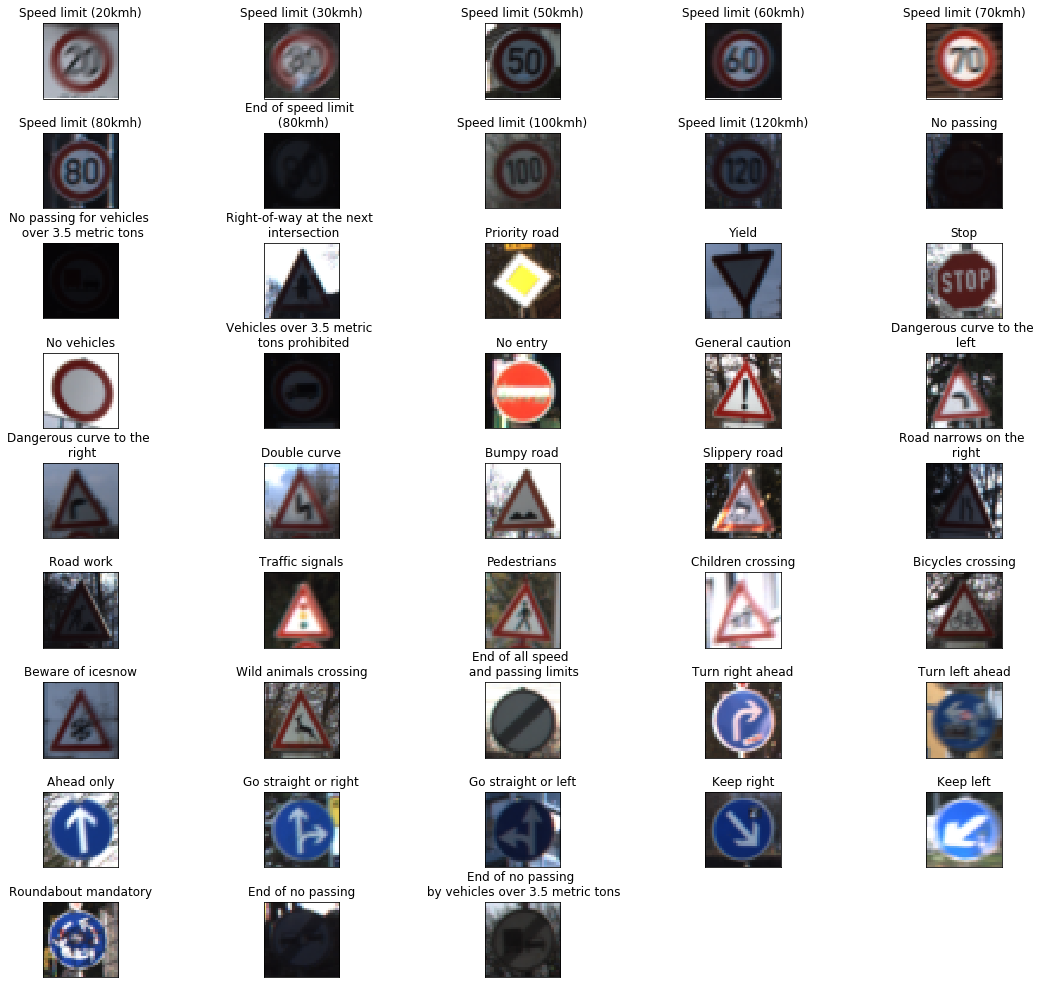
\includegraphics{./test_images_output/All signs.png}
\caption{All\%20signs.png}
\end{figure}

Let's now see some random images from the dataset to see how images can
look like:

\begin{figure}
\centering
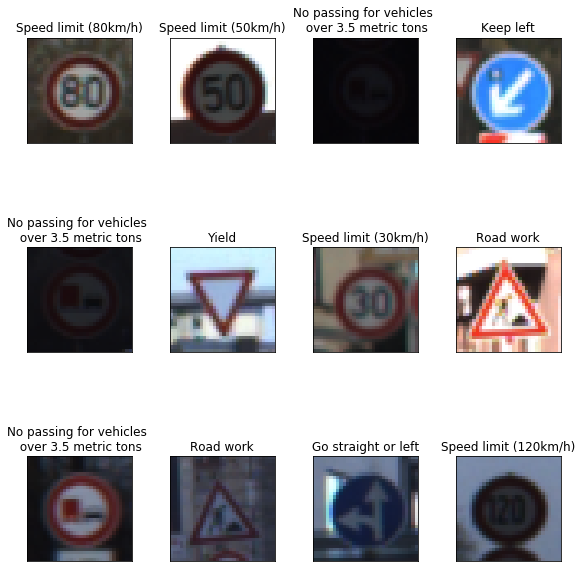
\includegraphics{./assets/random_dataset_images.png}
\caption{random\_dataset\_images.png}
\end{figure}

As we can see some images are dim others are bright, some are tilted and
others are blurred. That shows that our dataset images can vary in
quality and condition, this will be a recurring theme that we'll be
addressing in preprocessing and augmentation later in the project.

We got a nice random representation of our data which shows some of the
signs above.

Now onto more important things, in order for our model to train properly
and give good results our training dataset should have good
representation of each sign, ideally equal number of images but we'll
settle for a uniform one. Here we plot our training data distribution
which shows how many occurrences each class (sign) is in the training
dataset:

\begin{figure}
\centering
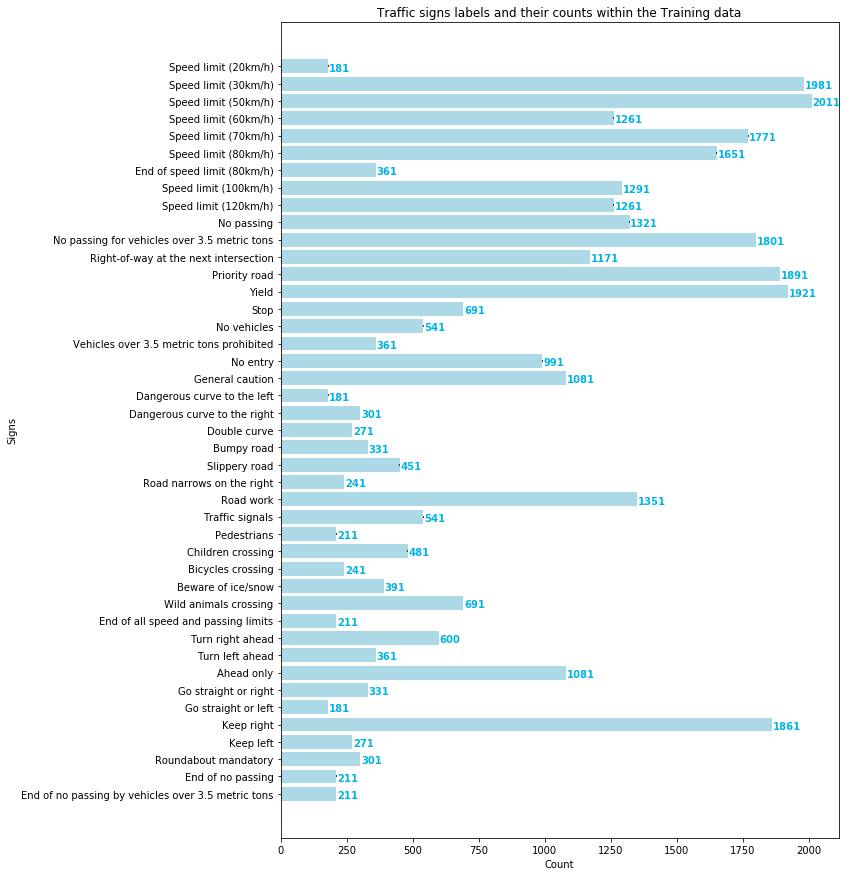
\includegraphics{./assets/classes_table.png}
\caption{classes\_table.png}
\end{figure}

\textbf{Conclusion:} as we can see from the graph above our training
dataset is highly skewed towards some classes while other classes have
really low number of images.For example, \textbf{Speed limit (50km/h)}
has the highest count of \textbf{2,011} images while \textbf{Go straight
or left} has the lowest count of \textbf{181}. This will make our model
biased towards signs with higher image counts and maybe it wont be able
to correctly classify signs with counts below 300 all the time.

    \hypertarget{design-and-test-a-model-architecture}{%
\section{Design and Test a Model
Architecture}\label{design-and-test-a-model-architecture}}

\begin{center}\rule{0.5\linewidth}{\linethickness}\end{center}

Here we explore different techniques to best preprocess our dataset and
get it ready for training. We gained inspiration from the \textbf{LeNet}
and other image classification models to create our model.

    \hypertarget{preprocessing}{%
\subsection{\#\# 1.Preprocessing}\label{preprocessing}}

Here are the preprocessing techniques that we explored and implemented
on our dataset:

\begin{itemize}
\tightlist
\item
  Data Shuffling
\item
  Normalization (Mean Normalization)
\item
  Grayscaling
\item
  Image Enhancement (sharpness)
\item
  Image Correction (Lighting)
\item
  Image Augmentation (Rotation, skewing, blurring)
\end{itemize}

    \hypertarget{data-shuffling}{%
\subsubsection{Data shuffling}\label{data-shuffling}}

So as it stands our training dataset images are ordered as we'll see in
the first 12 images here: 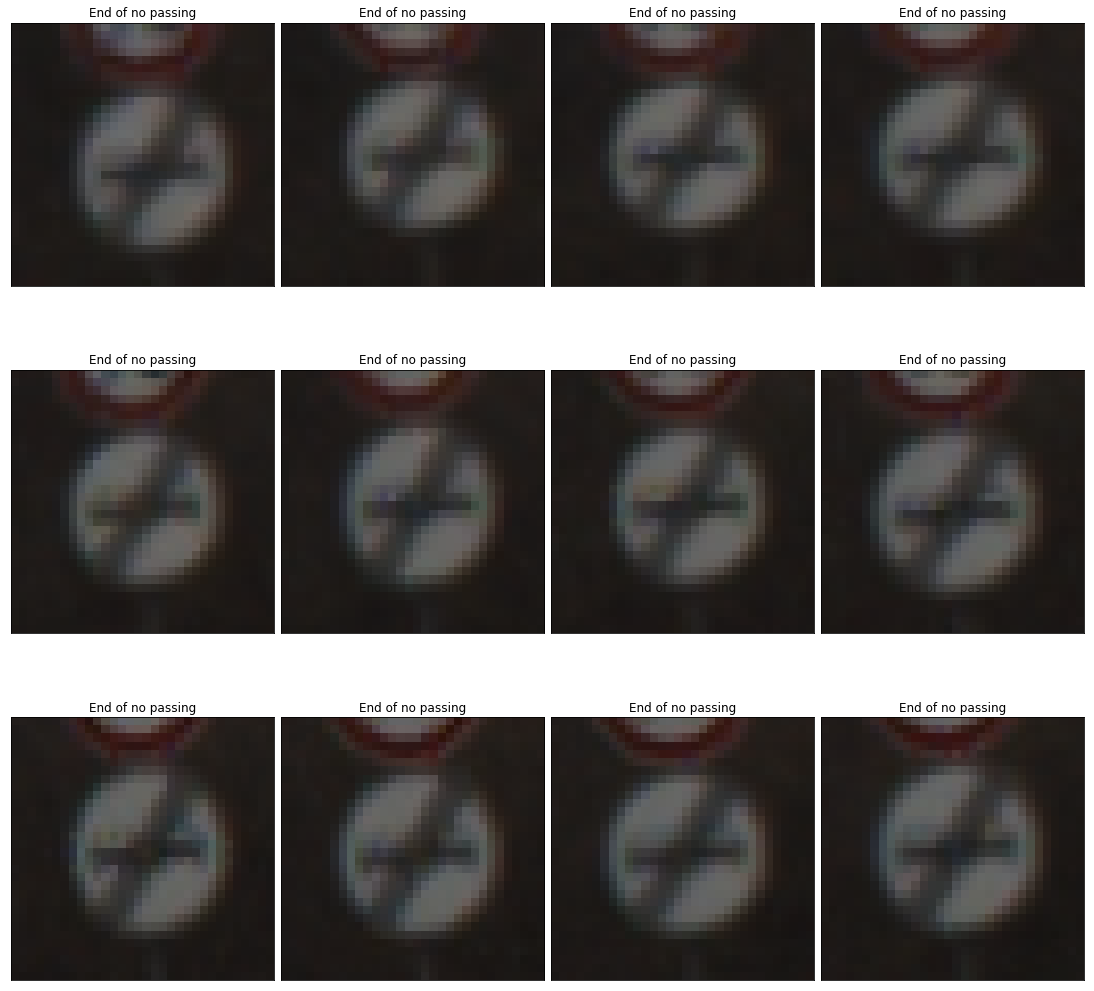
\includegraphics{./assets/first_12_images.png}
So we shuffled our data using the \texttt{shuffle()} method of the
\texttt{sklearn} utils methods to shuffle our images and their labels,
and we got a better random representation of the dataset as we can see
below the first 12 images after shuffling:
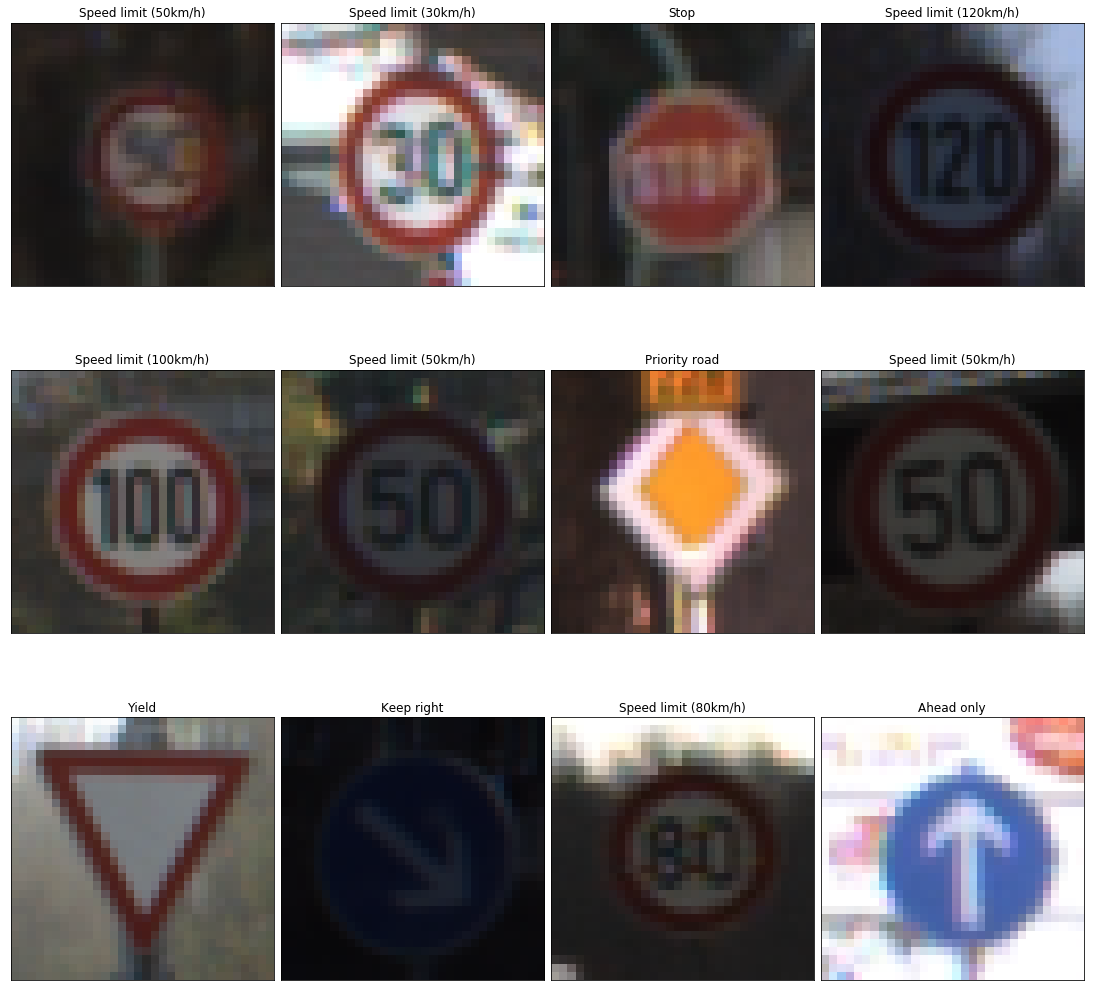
\includegraphics{./assets/random_first_12.png}

    \hypertarget{image-normalization}{%
\subsubsection{Image Normalization}\label{image-normalization}}

Normalization, feature scaling, or standardization is the last step in
preprocessing our dataset but we'll explain it here cause its going to
be mentioned a lot in the coming preprocessing techniques. It
standardizes our dataset features and bounds them to a range from
{[}0,1{]}, {[}-1,1{]}, or other which helps our model execute faster due
to this mathematical optimization. Here are two ways of normalizing our
data 1. An implementation of MINMAX which applies
\texttt{(pixel\ -\ 128)/\ 128} to every pixel of the image 2. Mean
normalization applying \texttt{(pixel\ -\ images\_mean)\ /\ images\_std}
to every pixel of the image

We opted for the second method where we apply \textbf{Mean
normalization} to all of our \emph{training}, \emph{validation}, and
\emph{test} datasets with the \texttt{images\_mean} and
\texttt{images\_std} as the training dataset's \texttt{mean} and
\texttt{standard\ deviation} respectively.

\begin{figure}
\centering
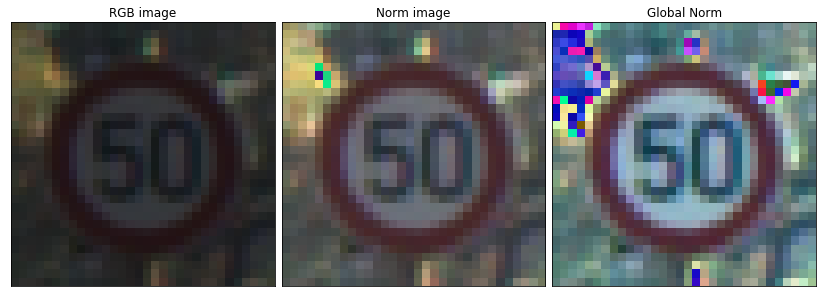
\includegraphics{./assets/RGB_normalized.png}
\caption{RGB\_normalized.png}
\end{figure}

Here is another example of a normal image and its globally normalized
counterpart:

\begin{longtable}[]{@{}cc@{}}
\toprule
Normal RGB image & Normalized Image\tabularnewline
\midrule
\endhead
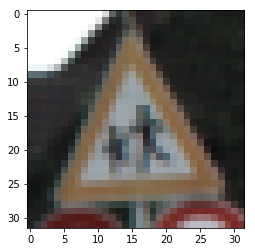
\includegraphics{./assets/normal_image.png} &
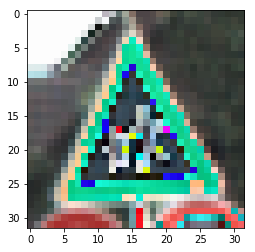
\includegraphics{./assets/normalized_image.png}\tabularnewline
\bottomrule
\end{longtable}

    \hypertarget{grayscaling}{%
\subsubsection{Grayscaling}\label{grayscaling}}

\texttt{Grayscaling} the dataset images was a really a good choice for
we found out that gave clearer images for different lighting scenarios,
it also normalizes well and doesn't lose information or create artifacts
like in the \texttt{RGB} images as we'll see in the images below:

\begin{figure}
\centering
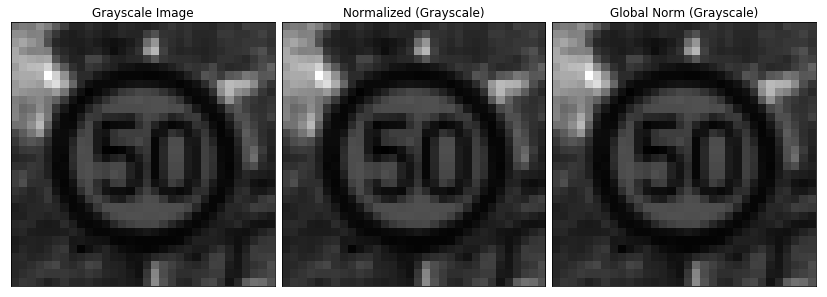
\includegraphics{./assets/normalized_grayscale.png}
\caption{normalized\_grayscale.png}
\end{figure}

So as a result we used \texttt{Grayscaled} images not only for the
benefits mentioned above but also because it enables us to to apply th
contrast adjustments techniques that we'll mention in the next section.

    \hypertarget{image-lighting}{%
\subsubsection{Image Lighting}\label{image-lighting}}

We tried out three techniques to correct the image lighting by adjusting
its contrast, these techniques are: * Adaptive Thresholding * Histogram
equalization * Adaptive Histogram equalization

These techniques were applied using \textbf{OpenCV} \texttt{cv2} module
and their implementation is in the
\href{./imageutils.py}{\texttt{imageutils.py}} file.

\hypertarget{adaptive-thresholding}{%
\paragraph{Adaptive Thresholding}\label{adaptive-thresholding}}

Adaptive thresholding is a technique used to emphasize image edges
regardless of the lighting condition, here are the resulted images:

\begin{figure}
\centering
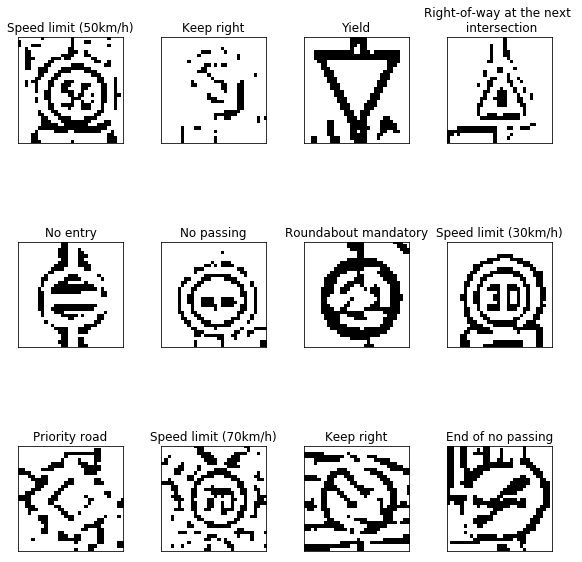
\includegraphics{./assets/adaptive_thresholding.png}
\caption{adaptive\_thresholding.png}
\end{figure}

While adaptive thresholding removes much of the image noise it also
removes a lot of some signs features, so we moved on to another
technique.

\hypertarget{histogram-equalization}{%
\paragraph{Histogram Equalization}\label{histogram-equalization}}

Histogram equalization is a technique that transforms the image to a
more bright if it was dark and vise versa, this technique maps image
pixels from one end of the spectrum (bright or dark) to the full range
of the image. This equalization makes sure that the image makes use of
its full light spectrum (contrast) so images appear more clear, it gives
us uniform lighting over all of the image pixels. It does this by
equalizing all pixel intensities to with the global image intensity.

\begin{figure}
\centering
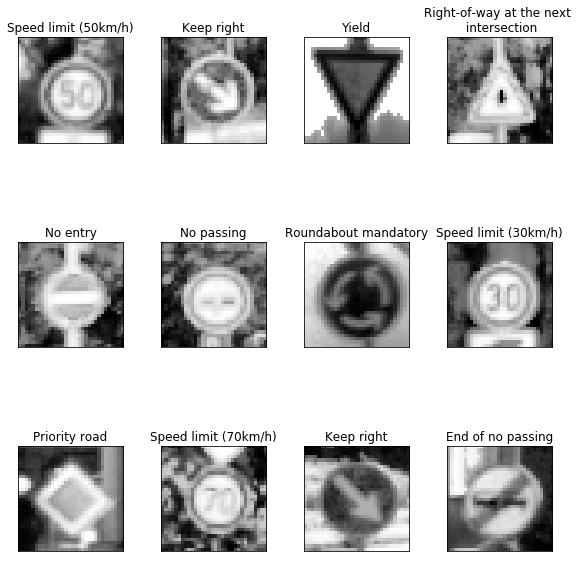
\includegraphics{./assets/histogram_equalization.png}
\caption{histogram\_equalization.png}
\end{figure}

Most of our images now appear clearer especially the low lit and low
contrast ones, but in the process of lighting these images up we
sacrificed some of their features. Some of the images lost their
definition, thats why we then applied the Adaptive Histogram
Equalization which should deal with this issue.

\hypertarget{adaptive-histogram-equalization-calhe}{%
\paragraph{Adaptive Histogram Equalization
(CALHE)}\label{adaptive-histogram-equalization-calhe}}

This is the Adaptive version of the Histogram equalization Contrast
Limited Adaptive Histogram Equalization CALHE for short, which limits
the contrast applied to each pixels by its neighboring pixels, so pixels
cant be affected by really bright or dim pixels that are not even near
them. This technique needs a filter or a grid size of how far from a
pixel should we consider neighbors, in our implementation we chose a
\texttt{3x3} grid size due to our small image size.

\begin{figure}
\centering
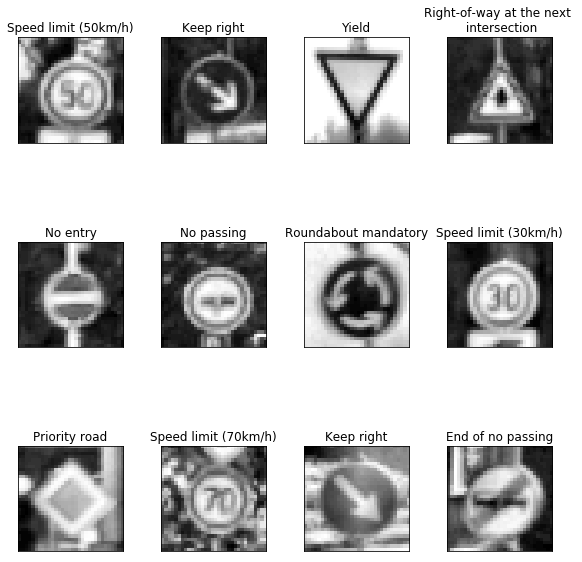
\includegraphics{./assets/calhe.png}
\caption{calhe.png}
\end{figure}

Now our image information is more defined and our image contrast it
decent and well distributed through the image, thats why we ended up
using this in our preprocessing pipeline.

\hypertarget{conclusion}{%
\paragraph{Conclusion:}\label{conclusion}}

We settled on the \texttt{CALHE} approach cause it correctly fixes our
image lighting situation which gives us clearer images to train our
network on, this also showed when we tested its accuracy versus
\texttt{Grayscale} and \texttt{RGB} as we'll see in the next sections.

\textbf{NOTE:}

You can find out more information on the \textbf{Histogram Equalization}
implementation in this {[}link{]}
(https://docs.opencv.org/3.1.0/d5/daf/tutorial\_py\_histogram\_equalization.html)
and you can also visit the
\href{https://en.wikipedia.org/wiki/Histogram_equalization}{wikipedia}
page for more information about the subject in general.

    \hypertarget{image-enhancement}{%
\subsubsection{Image Enhancement}\label{image-enhancement}}

After working a lot on the project and improving its techniques I got an
idea of enhancing the dataset images before applying any preprocessing
or augmentation, for the images are \texttt{32x32x3} and of blurry and
bad quality. So I added image sharpening to the preprocessing pipeline
that we execute on our \emph{training}, \emph{validation},
\emph{testing}, and any other image we train or infer. Here is an
example of image sharpening:
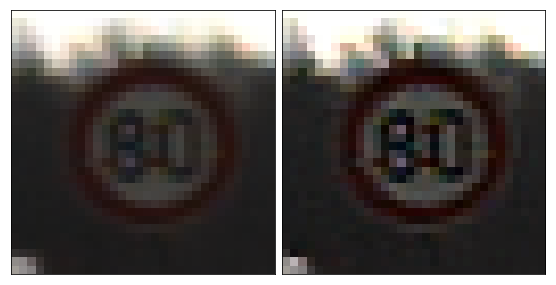
\includegraphics{./assets/image_sharpening.png}

As you can see the image is a bit clearer, but not by a huge factor
cause while trying out different factors on all the images some images
get too distorted and ignore main sing features, so by experimentation
we fount that \texttt{3} is a good sharpening factor.

We had 2 sharpening methods to choose from, one self made and the other
using \textbf{PIL's} (Python Image Library) \texttt{ImageEnhance} which
we opted for at the end because it proved more robust for all of our
dataset images.

    \hypertarget{rgbg}{%
\subsubsection{RGBG}\label{rgbg}}

We also explored the possibility of combining the Colored and Gray
channels, so we can get the combined benefits of the color information
in the {R}{G}{B} and the contrast CALHE equalized {Gray} in one image of
shape \texttt{32x32x4}. We'll see below in the approach section how did
this workout.

    \hypertarget{image-augmentation}{%
\subsubsection{Image Augmentation}\label{image-augmentation}}

Our dataset is class counts are imbalanced, some labels have more than
\textbf{1500} images while others have fewer than \textbf{500} images
and ones have as low as \textbf{181} images. This skewed representation
will influence our model to bias its classification towards classes with
higher number of images, and it'll decrease the probability of correctly
classifying low numbered images. In other works this will teach our
model to ``overfit'' the higher number labels, which results in bad
model generalization on all labels which will lead to poor accuracies
and ultimately a bad classifier.

In a perfect world we can solve this by getting more data, but here in
reality we'll have to create our own by augmenting our existing dataset
to get more versions of it. The augmentations that we applied were ones
that are applicable to the context of the dataset like rotate, add
noise, blur, brighten, etc..

Here are possible real world conditions for traffic signs that we might
be able to augment: * Low resolution images * lighting conditions
(saturations, low-contrast) * motion-blur * sunglare * Shade * physical
damage * colors fading * graffiti * point of view or perspective

So Lets create our own augmentations that replicates some of the
conditions listed above, we'll apply augmentations to replecate some of
the real world conditions that can affect the traffic signs.

\begin{itemize}
\tightlist
\item
  \texttt{blur\_image()} to replicate motion-blur from video extracted
  images or bad quality
\item
  \texttt{augment\_image\_pov} to replicate different perspectives or
  points of view of the image taken
\item
  \texttt{rotate()} to replicate physical damage or camera rotation
\item
  \texttt{bright\_dim\_image} to replicate different lighting conditions
\item
  \texttt{fade\_color()} to replicate physical damage and fading paint
\end{itemize}

Below we used techniques from multiple libraries and modules like
\texttt{scipy.ndimage}, \texttt{openCV}, \texttt{skimage.transform},
\texttt{PIL}, and own implementation, all of these methods are
implemented in the \href{imageutils.py}{\texttt{imageutils.py}} file.

\hypertarget{old-augmentation}{%
\paragraph{Old Augmentation}\label{old-augmentation}}

We started out with just a handful of augmentations and even some of
them like the rotate gave dark images, here is the first version of
image augmentations that we used:

\begin{figure}
\centering
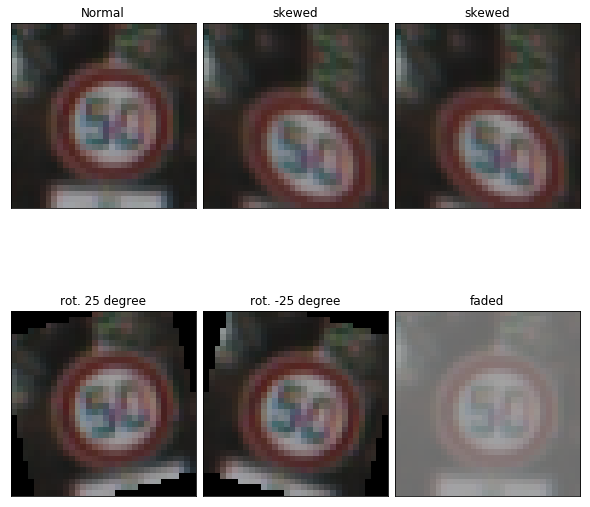
\includegraphics{./assets/augmented_images.png}
\caption{augmented\_images.png}
\end{figure}

\hypertarget{new-augmentation}{%
\paragraph{New Augmentation}\label{new-augmentation}}

Then after some search and coding we made another larger and more
meaningful augmentations which we ended up using in our final model, we
also applied them on \textbf{CALHE} images just to save some time
because we're going to convert them anyway.

Here are the new and improved image augmentations:

\begin{figure}
\centering
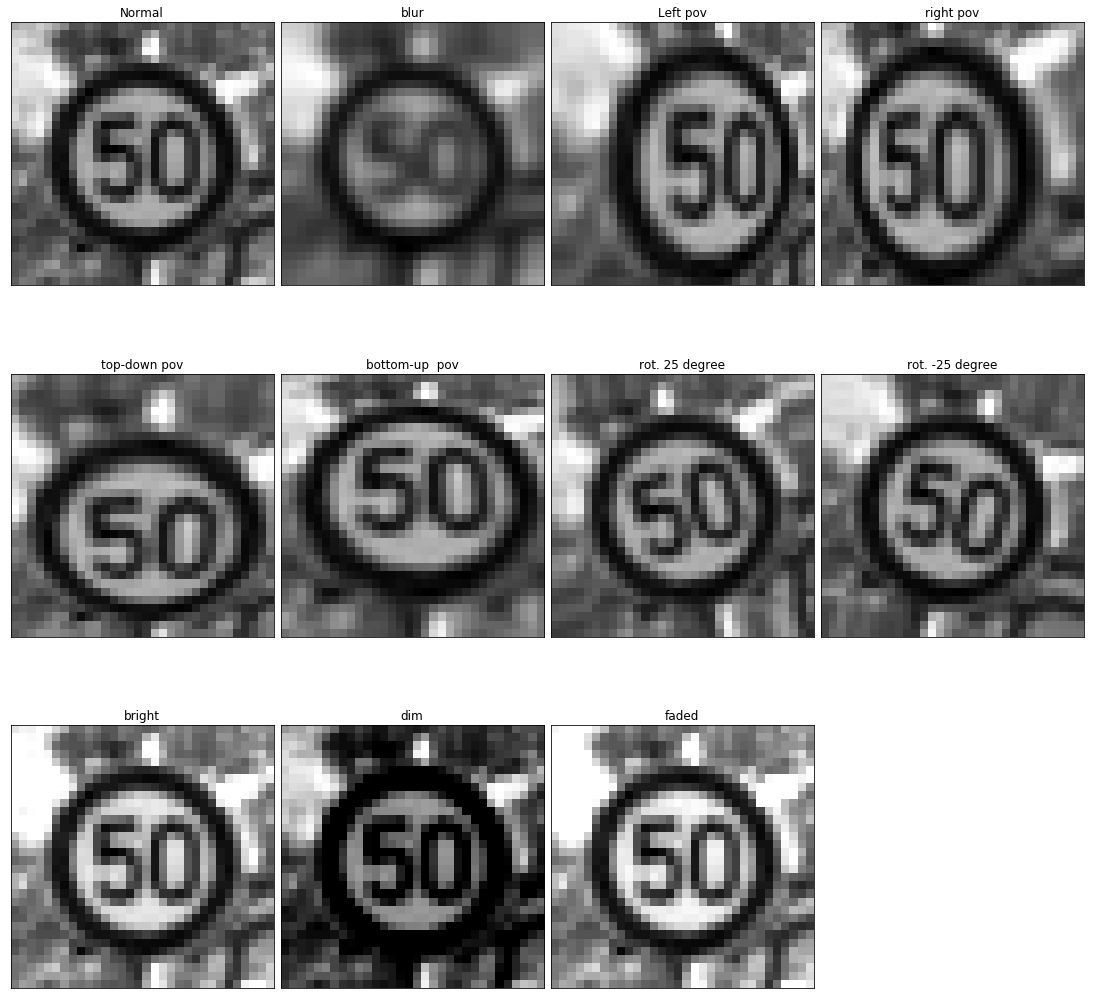
\includegraphics{./assets/image_aug.png}
\caption{image\_aug.png}
\end{figure}

As you can see these augmentations are way better than the original we
also improved the \texttt{rotate()} implementation as you can see above.

We applied these 10 augmentations relatively to images that need more
data representation like \textbf{Speed limit (20km/h)} and \textbf{Go
straight or left} which increased their image counts significantly.

This addition of meaningful real world augmentations will balance our
dataset skewed representation which will create a more robust traffic
signs classifier, notice that we didn't apply these augmentations to all
our classes thats because if we do that we're just scaling up the
imbalanced data representation and will end up in the same place we
started. We'll talk more about the actual values and how the
distribution looks in the approach section.

    \hypertarget{preprocess-pipeline}{%
\subsubsection{Preprocess Pipeline}\label{preprocess-pipeline}}

Here is the final preprocessing pipeline: 1. Enhance all images 2.
Convert all images to \textbf{CALHE}, which include converting to
\textbf{Grayscale} first. 3. Apply \emph{relative} augmentation to our
training dataset 3. Then finally apply normalization with the new images
mean and standard deviation to all sets

In the course of finding the optimal pipeline we reordered these steps
and ended up with this variation. We created 2 main methods
\texttt{preprocess()} and \texttt{augment()} in the project
\href{Traffic_Sign_Classifier.ipynb}{notebook}, these methods call
methods from the \href{imageutils.py}{\texttt{imageutils}} module that
you can go and explore how they work.

\hypertarget{image-enhancements}{%
\paragraph{1. Image Enhancements}\label{image-enhancements}}

So we first \textbf{enhanced} all of our images in \emph{training,
validation, and test} for the purpose of training and evaluation.

\hypertarget{calhe}{%
\paragraph{2. CALHE}\label{calhe}}

Then we converted all images to \textbf{Grayscale} then equalized them
using \textbf{CALHE}.

\hypertarget{relative-augmentation}{%
\paragraph{3. Relative Augmentation}\label{relative-augmentation}}

Then we applied \textbf{relative} augmentation only on our training
dataset; relative augmentation here means that we only augmented classes
with image count less that a \emph{Threshold}. Our threshold was
\textbf{1600} images, so our method went through our classes and found
classes with image counts less than \textbf{1600} images then it applied
augmentations on these classes for them to reach that threshold. We
tuned our threshold several times first we started with the
distribution's mean which was \textbf{810}, but the data generated
wasn't enough for low count classes, then with some trial and error we
got the best results using the value mentioned above.

Here is the result after applying the relative augmentation:

\begin{figure}
\centering
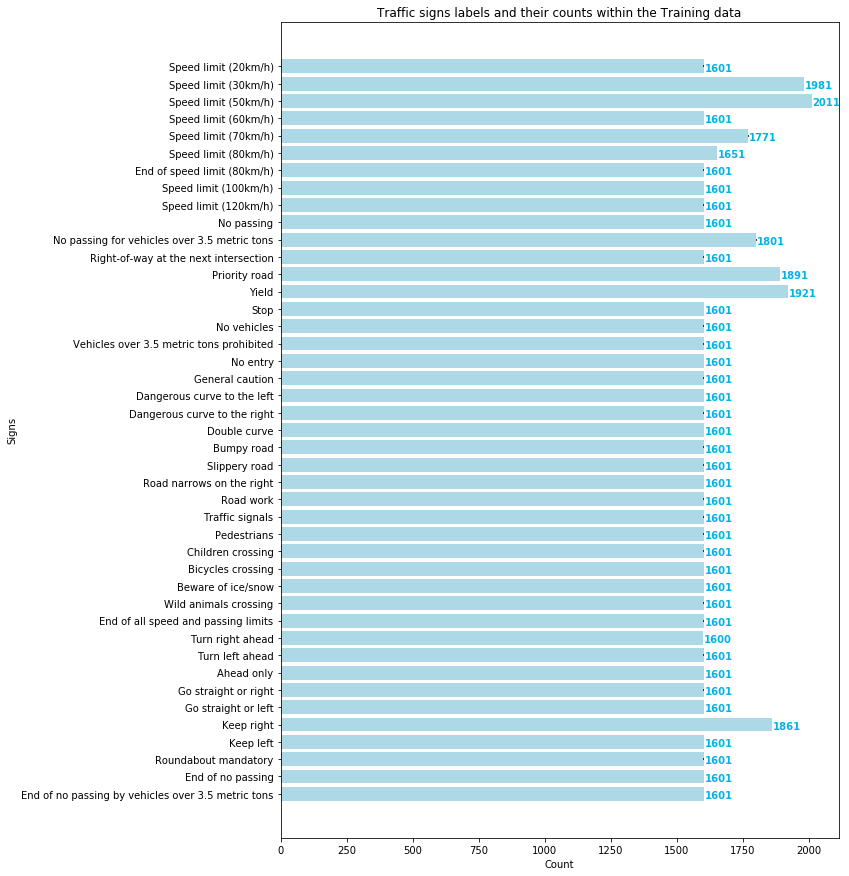
\includegraphics{./assets/augmented_data_distribution.png}
\caption{augmented\_data\_distribution.png}
\end{figure}

So by doing so we now have a more uniform distribution and close to
equal image representation that should eliminate the huge bias that we
first had in our data. This new distribution has a \emph{mean} of
\textbf{1,649} more than twice the original \textbf{810}, and \textbf{Go
straight or left} now has \textbf{1,601} images so does most of the
classes. This increased the class with the lowest number \textbf{181} to
\textbf{1,601} a 9 fold increase of meaningful image variation, apart
from solving our imbalanced distribution problem this increased our
\textbf{training} dataset from \textbf{34,799} to \textbf{70,879} thats
more than twice our original dataset size. These two new improvements
that resulted from our approach to data augmentation will give us a more
robust classifier.

\hypertarget{data-normalization}{%
\paragraph{4. Data Normalization}\label{data-normalization}}

As we said before normalization or standardization is a process of range
binding our image data to low float values like {[}-1,1{]} to
\emph{mathematically optimize} our data and make it easy for our machine
to execute hardware intensive operations on such a huge number of data.
So after we were done with all of the other preprocessing operations we
applied \emph{global mean} standardization on all of our
datasets(training, validation, and testing) using the \emph{mean} and
\emph{standard deviation} of the new \textbf{CALHE} augmented images.
Then we fed our datasets to the model that we're going to talk about in
the next section.

\hypertarget{note-this-pipeline-is-applied-to-our-training-validation-testing-and-any-other-images-that-use-the-model-for-inference.}{%
\paragraph{NOTE: This pipeline is applied to our training, validation,
testing, and any other images that use the model for
inference.}\label{note-this-pipeline-is-applied-to-our-training-validation-testing-and-any-other-images-that-use-the-model-for-inference.}}

    \hypertarget{model-architecture}{%
\subsection{\#\# 2. Model Architecture}\label{model-architecture}}

Here is the model inspired by LeNet and other CNNs, its called MoNet
following the same convention used in LeNet the of course stands for
Model not the first 2 letters of my name ;).

\begin{figure}
\centering
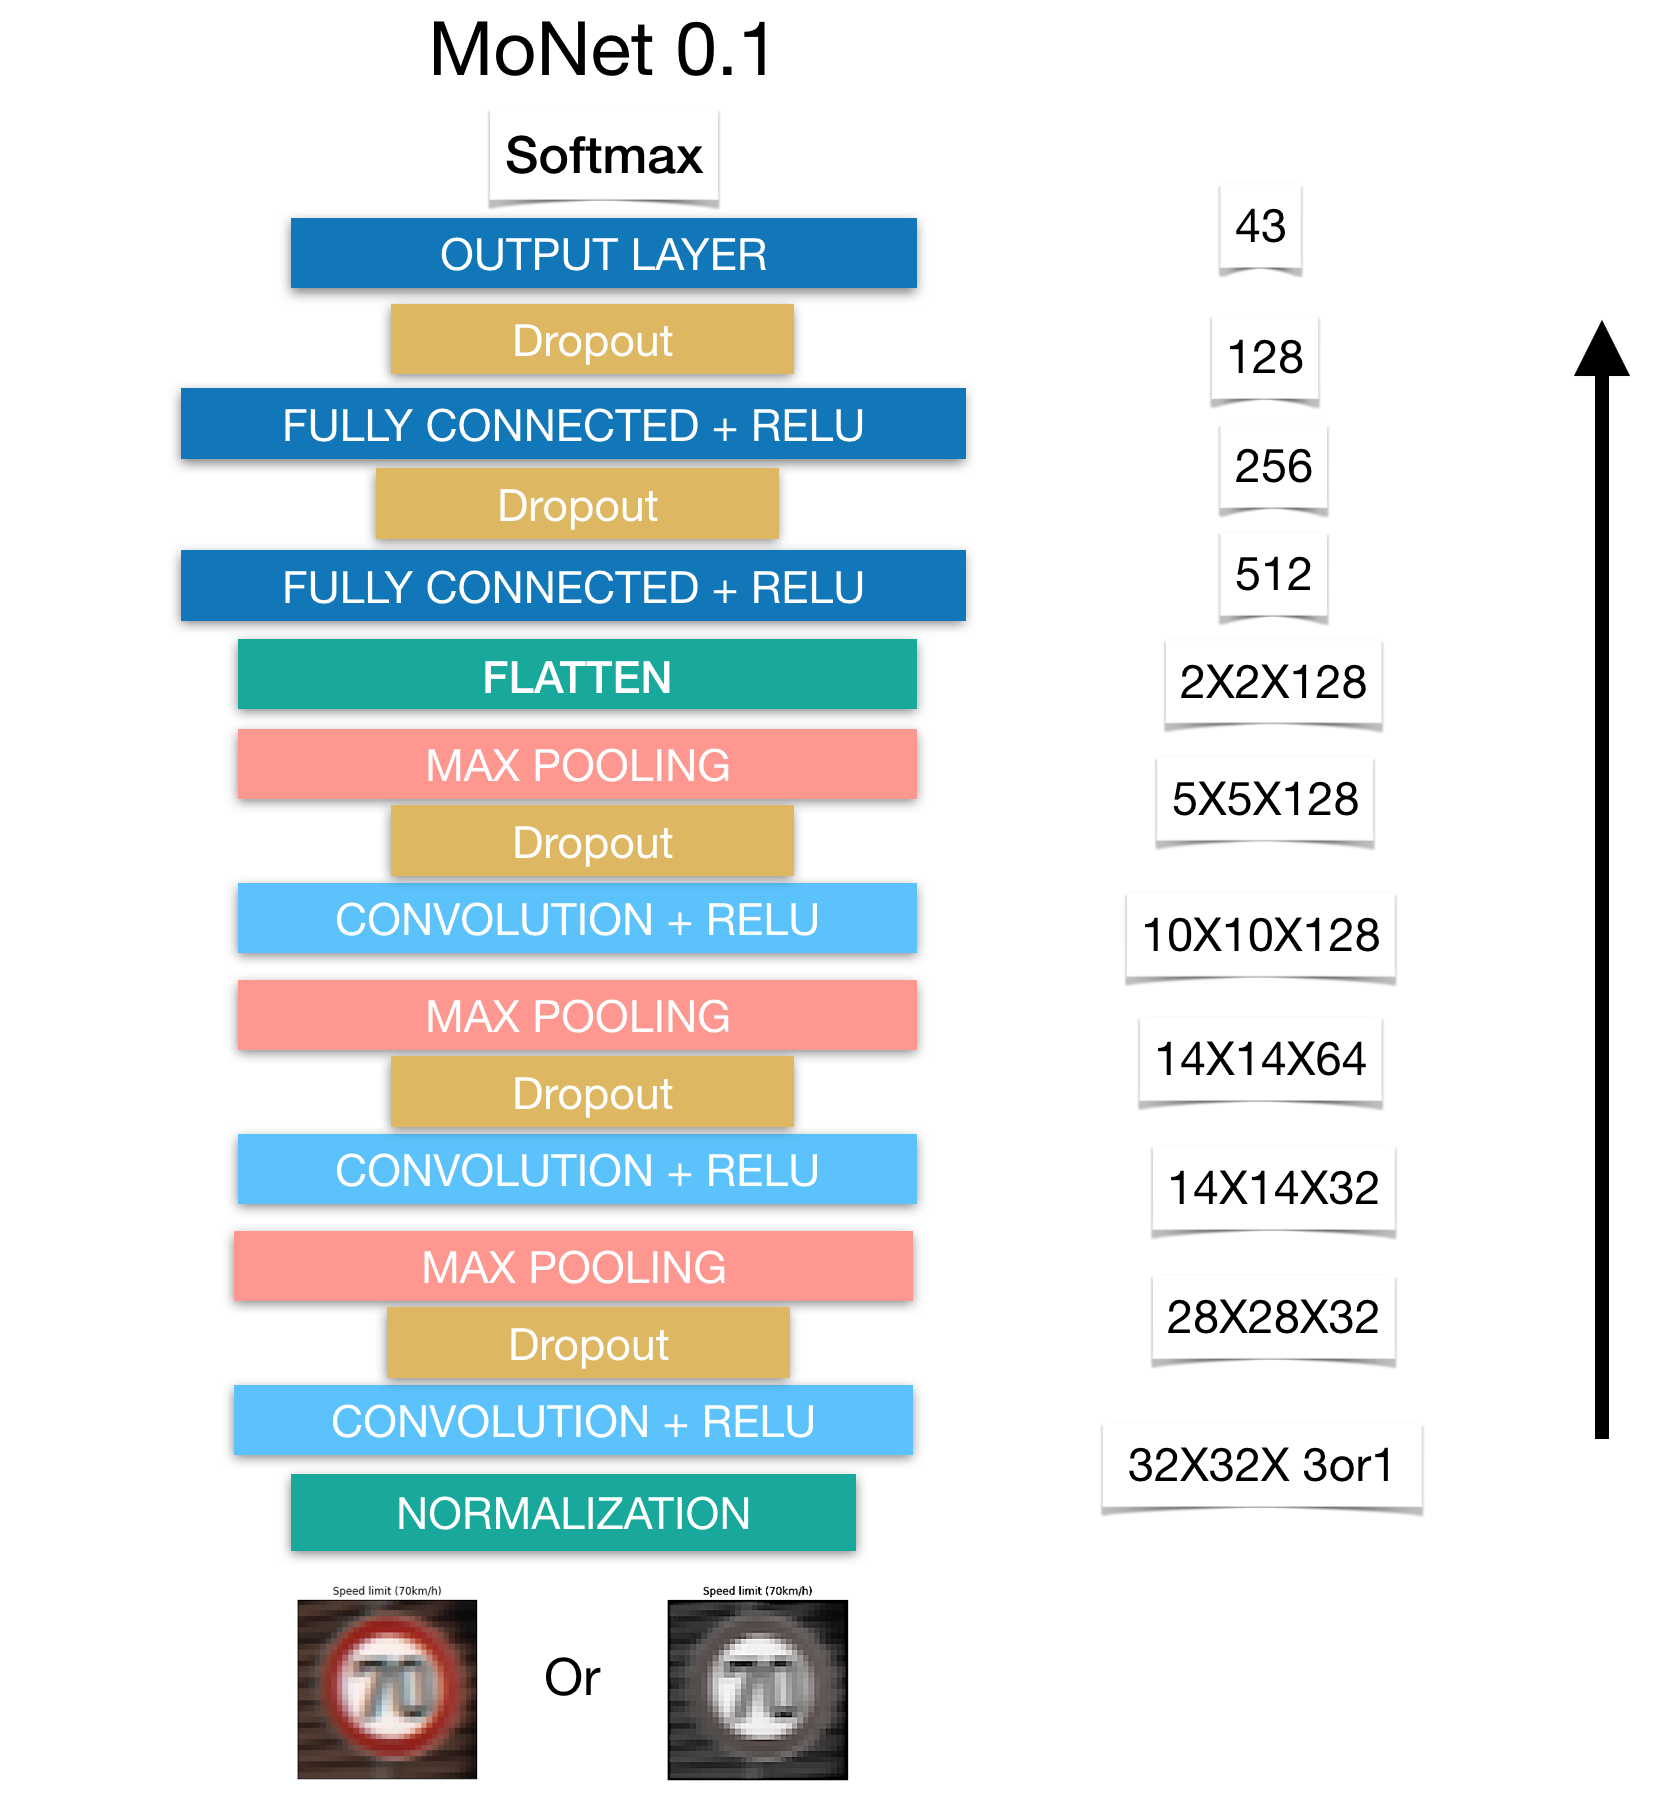
\includegraphics{./assets/MoNet_correct.png}
\caption{MoNet0.1.png}
\end{figure}

So as we can see its the same as the LeNet architecture with few key
differences, which are * One more \texttt{conv\_maxpool} layer (I
combined the convolutional and the maxpool in one method) * Deeper
filters to capture more information about the image * Deeper fully
connected layers * Dropout added after each convolutional and fully
connected layer to regularize our model

First I started with the LeNet model then I added a convolutional layer
which gave better results, then I started running different tests to get
a good depth for my network:

\begin{longtable}[]{@{}cc@{}}
\toprule
Layer & Description\tabularnewline
\midrule
\endhead
Input Image & Normalized CALHE 32x32x1 image\tabularnewline
Convolution 5x5 & 1x1 stride, VALID padding, outputs
28x28x32\tabularnewline
RELU & Non linearity activation function\tabularnewline
Dropout & Applies dropout of 0.75, 0.70, 0.65, 0.60, 0.55\tabularnewline
Max pooling & 2x2 stride, outputs 14x14x32\tabularnewline
Convolution 5x5 & 1x1 stride, VALID padding, outputs
10x10x64\tabularnewline
RELU & Non linearity activation function\tabularnewline
Dropout & Applies dropout of 0.75, 0.70, 0.65, 0.60, 0.55\tabularnewline
Max pooling & 2x2 stride, outputs 5x5x64\tabularnewline
Convolution 5x5 & 1x1 stride, SAME padding, outputs
5x5x128\tabularnewline
RELU & Non linearity activation function\tabularnewline
Dropout & Applies dropout of 0.75, 0.70, 0.65, 0.60, 0.55\tabularnewline
Max pooling & 2x2 stride, outputs 2x2x6128\tabularnewline
Flattening & Flattened the 2x2x128, output 512 feature
array\tabularnewline
Fully connected & Takes 512, and outputs 512\tabularnewline
Dropout & Applies dropout of 0.50\tabularnewline
Fully connected & Takes 512, and outputs 256\tabularnewline
Dropout & Applies dropout of 0.50\tabularnewline
Logits (Classifier) & Takes 256, outputs 43\tabularnewline
Cross Entropy loss & Softmax cross entropy\tabularnewline
AdamOptimizer & Optimize the model with a decaying learning
rate\tabularnewline
\bottomrule
\end{longtable}

    \hypertarget{training-the-model}{%
\subsection{\#\# 3. Training the Model}\label{training-the-model}}

\hypertarget{model-training}{%
\subsubsection{Model Training}\label{model-training}}

I used my personal PC to train, evaluate, and test the model, I used
\texttt{Tensorflow-GPU} which ran on an \textbf{NVIDIA GTX 980-ti} which
is a decently fast \emph{GPU} for training the model and its still good
at games. Though the \emph{GPU} is tough and performs fast operation,
however, training took a long time some of which too up to \texttt{3}
hours(augmented RGBG).

\hypertarget{model-hyperparameters}{%
\subsubsection{Model HyperParameters}\label{model-hyperparameters}}

A model's hyperparameters are the way we tune and manage how are model
performs, and its essential that they get set correctly in order for the
model to give its optimal performance. We set and played around with
alot of parameter in this project and for the nature of its complexity
it took days to train the model on different variations which we'll be
seeing in the section below, but here are the hyperparameters that we
tuned in the course of this project:

\textbf{Batch size:} I started with a batch size of \texttt{128} which
is kind of the default for most machines, but it takes more time to
train especially after applying augmentation. So I ran tried and tested
on different multiples \texttt{256}, \texttt{512}, then stopped at
\texttt{1024} cause I felt that it was fast enough and didn't want to
compromise the \textbf{mini- batch SGD} and overfit.

\textbf{Epochs:} At the start I used \texttt{30\ epoch} which is funny
when I look back at it, then when I started adding more depth, lower
learning rate, and dropout to my network it became clear that I needed a
bigger number so I went with \texttt{50} then \texttt{100},
\texttt{500}, \texttt{1000}, and even \texttt{2000} which takes 3.5
hours to train. mainly I used lower number of epoch like \texttt{100} or
\texttt{500} to validate variation of parameters that I was testing then
I used the heavy hitters \texttt{1000}, and \texttt{2000} to get the
best accuracy possible, it was mainly a difference of less that
\texttt{1\%} but I was striving for the best accuracy.

\textbf{learning rate:} Here I started with \texttt{0.001} a low number
from the get go because you can never go wrong with a low learning rate
it will always converge to the (Not always), hopefully to the global
minimum. However, we have to be wary of not overfitting, thats why I
applied \textbf{dropout} to the network to keep the network from
overfitting the training set. After some testing I even lowered the
learning rate to \texttt{0.0001} which yielded better morestable
results.

I also got to played around with the \emph{optimizer} and ultimately
chose the \texttt{AdamOptimizer} which is an implementation of the
\href{https://arxiv.org/pdf/1412.6980.pdf}{Adam algorithm} of the
\textbf{Stochastic Gradient decent} created by \emph{Diederik P.
Kingma}, and \emph{Jimmy Ba}. This \texttt{tf.train.AdamOptimizer()} is
better than the \texttt{tf.train.GradientDescentOptimizer()} because it
calculates the moving mean or \textbf{momentum} that automatically
calculates the \textbf{adaptive learning rate} and increases or
decreases it to get the optimal learning rate. However the algorithm
takes more time due to the underlying computations, but it deals with
fine tuning the learning rate to converge. You can learn all about the
algorithm and its implementation
{[}here{]}.(https://www.tensorflow.org/api\_docs/python/tf/train/AdamOptimizer)

\textbf{Friendly advice: don't change the epsilon parameter if you don't
completely understand it}

    \hypertarget{training-approach}. The model was tested and improved several times against
many

I did some exhaustive testing to see effect each small variation has on
the end result, and by exhaustive I mean that my \emph{GPU} worked like
it never ever did before. First I tried the effect different
\textbf{colors spaces} have on the training and validation accuracies, I
also added in CALHE (Adaptive Histogram Equalization) into the mix to
see how well it does against RGB and grayscale, I also t. I also
explored different \textbf{normalization} techniques like MINMAX
normalization and global mean normalization. I added
\textbf{augmentation} and compared the results to the normal data before
augmentation. Then I added \textbf{dropout}, changed its values, and
even removed it all together from some layers. I experimented with other
\textbf{non-linear activations} like leaky-relu and elu. I also tried
out to combine the RGB and the CALHE layers \textbf{(RGBG)} which got me
a \textbf{32x32x4} image. Below I'll be showing the result of these
experiments and the results of the most successful run.

\textbf{NOTE:} The initial model had \texttt{3} \texttt{convolutional}
of depths \texttt{{[}8,\ 16,\ 32{]}} and \texttt{2}
\texttt{fully-connected} layers of depths \texttt{{[}128,\ 64{]}}, then
a \texttt{logits} layer of depth \texttt{43} the number of classes.

\hypertarget{normalization}{%
\subsubsection{Normalization}\label{normalization}}

normalization on \texttt{2} color variations (RGB and Grayscale), the
initial results were somehow disappointing cause the validation accuracy
actually dropped after applying data normalization as we can see in the
graphs below.

30 Epochs:

\hypertarget{colored-image}{%
\paragraph{Colored Image}\label{colored-image}}

\begin{longtable}[]{@{}lcc@{}}
\toprule
\begin{minipage}[b]{0.24\columnwidth}\raggedright
Type\strut
\end{minipage} & \begin{minipage}[b]{0.34\columnwidth}\centering
Normal Image\strut
\end{minipage} & \begin{minipage}[b]{0.34\columnwidth}\centering
Normalized Image\strut
\end{minipage}\tabularnewline
\midrule
\endhead
\begin{minipage}[t]{0.24\columnwidth}\raggedright
Accuracy\strut
\end{minipage} & \begin{minipage}[t]{0.34\columnwidth}\centering
Training= 97.8\% Validation= 91.8\%\strut
\end{minipage} & \begin{minipage}[t]{0.34\columnwidth}\centering
Training = 99.1\% Validation = 81.0\%\strut
\end{minipage}\tabularnewline
\begin{minipage}[t]{0.24\columnwidth}\raggedright
Graphs\strut
\end{minipage} & \begin{minipage}[t]{0.34\columnwidth}\centering
\strut
\end{minipage} & \begin{minipage}[t]{0.34\columnwidth}\centering
\strut
\end{minipage}\tabularnewline
\bottomrule
\end{longtable}

\hypertarget{grayscale}{%
\paragraph{Grayscale}\label{grayscale}}

\begin{longtable}[]{@{}lcc@{}}
\toprule
\begin{minipage}[b]{0.24\columnwidth}\raggedright
Type\strut
\end{minipage} & \begin{minipage}[b]{0.34\columnwidth}\centering
Grayscale Image\strut
\end{minipage} & \begin{minipage}[b]{0.34\columnwidth}\centering
Normalized Grayscale Image\strut
\end{minipage}\tabularnewline
\midrule
\endhead
\begin{minipage}[t]{0.24\columnwidth}\raggedright
Accuracy\strut
\end{minipage} & \begin{minipage}[t]{0.34\columnwidth}\centering
Training= 96.0\% Validation= 88.0\%\strut
\end{minipage} & \begin{minipage}[t]{0.34\columnwidth}\centering
Training = 99.5\% Validation = 81.6\%\strut
\end{minipage}\tabularnewline
\begin{minipage}[t]{0.24\columnwidth}\raggedright
Graphs\strut
\end{minipage} & \begin{minipage}[t]{0.34\columnwidth}\centering
\strut
\end{minipage} & \begin{minipage}[t]{0.34\columnwidth}\centering
\strut
\end{minipage}\tabularnewline
\bottomrule
\end{longtable}

However, this was training the model for just \texttt{30} epoch and
thought to increase the number of epochs, but I noticed that the
training value increases and the validation accuracy decreases that and
the \emph{zigzag} shape of the graphs meant that the model was
\textbf{overfitting}. This makes sense since normalization speeds up
convergence, I asserted this by testing over \texttt{100} epochs as
shown in the table below:

\begin{longtable}[]{@{}lcc@{}}
\toprule
\begin{minipage}[b]{0.24\columnwidth}\raggedright
Type\strut
\end{minipage} & \begin{minipage}[b]{0.34\columnwidth}\centering
Normal accuracy\strut
\end{minipage} & \begin{minipage}[b]{0.34\columnwidth}\centering
Normalized accuracy\strut
\end{minipage}\tabularnewline
\midrule
\endhead
\begin{minipage}[t]{0.24\columnwidth}\raggedright
Color\strut
\end{minipage} & \begin{minipage}[t]{0.34\columnwidth}\centering
Training = 99.2\% Validation= 94.0\%\strut
\end{minipage} & \begin{minipage}[t]{0.34\columnwidth}\centering
Training = 99.8\% Validation = 64.6\%\strut
\end{minipage}\tabularnewline
\begin{minipage}[t]{0.24\columnwidth}\raggedright
Grayscale\strut
\end{minipage} & \begin{minipage}[t]{0.34\columnwidth}\centering
Training = 99.4\% Validation = 93.4\%\strut
\end{minipage} & \begin{minipage}[t]{0.34\columnwidth}\centering
Training = 99.8\% Validation = 73.8\%\strut
\end{minipage}\tabularnewline
\bottomrule
\end{longtable}

So it turns out to be the same as \texttt{30} epoch with the only
exception being the \textbf{CALHE} with high numbers in both tests. It
seamed that the model was just over fitting, but as we'll see below the
model's depth had a lot to do with it.

\hypertarget{depth}{%
\subsubsection{Depth}\label{depth}}

I increased the network depth form the initial depths to
\texttt{{[}32,\ 64,\ 128{]}} for the \texttt{convolutional} layers
filters, and \texttt{{[}512,\ 256{]}} for the \texttt{fully-connected}
layers. This significantly deeper network did the trick and gave better
result as and the deeper network in solving the solving the
\textbf{overfitting} issue. Here are the results of the network depth on
\textbf{RGB} and \textbf{Grayscale} images.

\hypertarget{colored-image-1}{%
\paragraph{Colored Image}\label{colored-image-1}}

\begin{longtable}[]{@{}lcc@{}}
\toprule
\begin{minipage}[b]{0.24\columnwidth}\raggedright
Type\strut
\end{minipage} & \begin{minipage}[b]{0.34\columnwidth}\centering
Normal Image\strut
\end{minipage} & \begin{minipage}[b]{0.34\columnwidth}\centering
Normalized Image\strut
\end{minipage}\tabularnewline
\midrule
\endhead
\begin{minipage}[t]{0.24\columnwidth}\raggedright
Accuracy\strut
\end{minipage} & \begin{minipage}[t]{0.34\columnwidth}\centering
Training= 99.8\% Validation= 92.0\%\strut
\end{minipage} & \begin{minipage}[t]{0.34\columnwidth}\centering
Training = 100.0\% Validation = 92.3.0\%\strut
\end{minipage}\tabularnewline
\begin{minipage}[t]{0.24\columnwidth}\raggedright
Graphs\strut
\end{minipage} & \begin{minipage}[t]{0.34\columnwidth}\centering
\strut
\end{minipage} & \begin{minipage}[t]{0.34\columnwidth}\centering
\strut
\end{minipage}\tabularnewline
\bottomrule
\end{longtable}

\hypertarget{grayscale-1}{%
\paragraph{Grayscale}\label{grayscale-1}}

\begin{longtable}[]{@{}lcc@{}}
\toprule
\begin{minipage}[b]{0.24\columnwidth}\raggedright
Type\strut
\end{minipage} & \begin{minipage}[b]{0.34\columnwidth}\centering
Grayscale Image\strut
\end{minipage} & \begin{minipage}[b]{0.34\columnwidth}\centering
Normalized Grayscale Image\strut
\end{minipage}\tabularnewline
\midrule
\endhead
\begin{minipage}[t]{0.24\columnwidth}\raggedright
Accuracy\strut
\end{minipage} & \begin{minipage}[t]{0.34\columnwidth}\centering
Training= 100.0\% Validation= 94.1\%\strut
\end{minipage} & \begin{minipage}[t]{0.34\columnwidth}\centering
Training = 100.0\% Validation = 94.2\%\strut
\end{minipage}\tabularnewline
\begin{minipage}[t]{0.24\columnwidth}\raggedright
Graphs\strut
\end{minipage} & \begin{minipage}[t]{0.34\columnwidth}\centering
\strut
\end{minipage} & \begin{minipage}[t]{0.34\columnwidth}\centering
\strut
\end{minipage}\tabularnewline
\bottomrule
\end{longtable}

As we can see the network now achieves much higher accuracies and we can
also see that the normalized graph is a lot smoother now which is mainly
due to \textbf{overfitting}. I also tried out different weights for only
the \texttt{fully-connected} layers; for example,
\texttt{{[}256,\ 128{]}} but in the end the I settled on the combination
thats mentioned above.

Judging by the accuracy increase from this example test and others I
empirically derived that the \textbf{Grayscaled} images perform better
overall and that the \textbf{deeper}models out perform the shallower
ones, also we now need more epoch to train the model as it is deeper and
takes more time to train; however, we can see that our validation
accuracy doesn't change after about \texttt{40} epochs and our training
accuracy is near a \texttt{100\%} which meant that our model is
\textbf{overfiting} and not generalizing well on to the validation set.
Thats why I:

\begin{itemize}
\tightlist
\item
  Added dropout to prevent the model from overfitting
\item
  Getting more data through augmentation
\end{itemize}

\hypertarget{dropout}{%
\subsubsection{Dropout}\label{dropout}}

I applied dropout which is a regularization technique that prevents our
model from overfitting by setting a determined percentage of a layer's
weights which are randomly selected to 0, so the model cannot depend on
one feature or connection too much.

I applied \texttt{2} variations of dropout: 1. dropout of 0.5 keep
probability on only the fully connected layers 2. dropout of 0.75 and
0.5 keep probability on the convolutional and fully connected layers
respectively

The two variations gave close results over \texttt{100} epochs, but the
real difference was obvious over more epochs where the second variation
gave an increase of about \texttt{3\%}. So I chose the second variation
and after comparing both the \textbf{Grayscale} an the \textbf{CALHE}
versions, the \textbf{CALHE} preformed better than the \textbf{Grascale}
by about \texttt{2-3\%} validation accuracy, which made our validation
accuracy jump to \texttt{98.5\%} and our training accuracy to be close
to a \texttt{100\%}. Here is a graph of the the \textbf{CALHE} with
dropout over \texttt{500} epochs.

\begin{figure}
\centering
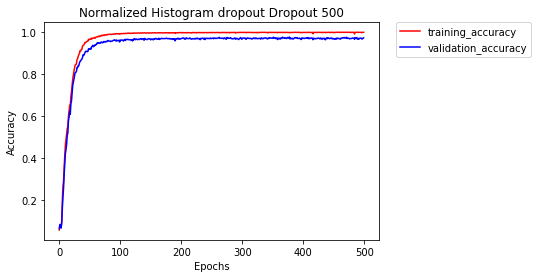
\includegraphics{./accuracies/finaltests/Normalized Histogram dropout Dropout 500.png}
\caption{Normalized\%20Histogram\%20dropout\%20Dropout\%20500.png}
\end{figure}

Now we can see a smooth close training and validation accuracies.

\hypertarget{augmentation} validation accuracy. I then proceeded
to apply \textbf{\emph{relative} data augmentation} which decreased the
accuracy for the first couple of epochs then slightly increased the
validation accuracy. It seemed that the addition of this new augmented
data which increased the training dataset size from \texttt{34,799} to
\texttt{63,000} images helped our model to learn better, this showed in
the slight increase of the in validation accuracy of \texttt{99\%}. Now
that we have really solid model that performs well on the Training and
validation set we can now turn our attention to the test set.

\hypertarget{improvement} which is an amazing result and way over the
required upper limit for this project. However, after looking into the
augmentation pipeline I noticed that some of the methods needed some
adjustments and I could add more augmentations to the images, so I added
more augmentations and improved on the existing ones and now the
training dataset size increased from \texttt{34,799} to \texttt{70,879},
but while the validation accuracy increased the test accuracy actually
decreased to \texttt{95\%}. That increase of dataset size and decrease
of accuracy made me think of changing the dropout to reduce overfitting
as we'll see next.

\hypertarget{different-variations}{%
\subsubsection{Different variations}\label{different-variations}}

I proceeded to tweak the hyperparameters, dropout values, and added
image enhancements to increase the \textbf{test} accuracy, I saved each
variation of the \texttt{MoNet} as a reference for comparison and then
chose the best one. Here are the variations and their results:

\textbf{NOTE:} All the models were trained for 2000 epochs with a batch
size of 1024, and a 0.0001 learning rate.

\hypertarget{monet-0.1.1} Training accuracy * \texttt{98.8\%}
Validation accuracy * \texttt{95.8\%} Test accuracy.

\hypertarget{monet-0.1.2} to better generalize given the high epoch count.

We lowered the convolutional layer's dropout to \texttt{0.55} which is
the lowest we'll be doing in this project, this is to prevent the
network from over-fitting our training data over many epochs. The
importance of \textbf{dropout} is that it helps generalize the model
over the validation, test, or any example by randomly omitting 50\% (the
keep probability 100 - keep probability) of the layer's features by
setting their weights to zeros, this helps the network to be independent
of certain features and give notice to all features equally; for
example, if we have a feature like rounded corners and we assign high
weight to it all the time then it over shadows the other features
because we're just increasing its weight without giving chance for the
other features to get trained as well, but by adding a drop out we know
that we give every feature a change in training which will in turn
abstract some of the features that will help generalize to future edged
examples per se.

This variation increased our \textbf{test} accuracy by about
\texttt{2\%} as we can see below.

With results: * \texttt{99.9\%} Training accuracy * \texttt{99.4\%}
Validation accuracy * \texttt{97.5\%} Test accuracy.

\hypertarget{monet-0.1.3} and slightly decreased the validation accuracy.

\begin{itemize}
\tightlist
\item
  \texttt{99.9\%} Training accuracy
\item
  \texttt{98.8\%} Validation accuracy
\item
  \texttt{98.0\%} Test accuracy
\end{itemize}

\hypertarget{monet-0.1.4}. Here
we noticed no increase in the \textbf{test} accuracy but a slight
increase of about \texttt{0.8\%} for the \textbf{validation} accuracy.

\begin{itemize}
\tightlist
\item
  \texttt{99.9\%}Training accuracy
\item
  \texttt{99.4\%} Validation accuracy
\item
  \texttt{98.0\%}Test accuracy
\end{itemize}

\hypertarget{monet-0.1.5} isn't resulted by a good guess, but
consistent along at least 4 consecutive epochs.

\begin{itemize}
\tightlist
\item
  \texttt{99.9\%} Training accuracy
\item
  \texttt{99.5\%} Validation accuracy
\item
  \texttt{98.2\%} Test accuracy
\end{itemize}

\hypertarget{monet-0.1.6} for both the
\textbf{validation} and \textbf{test} accuracies.

\begin{itemize}
\tightlist
\item
  \texttt{99.9\%} Training accuracy =
\item
  \texttt{99.3\%} Validation accuracy
\item
  \texttt{98.1\%} Test accuracy
\end{itemize}

\hypertarget{monet-0.1.7} Training accuracy\\
\item
  \texttt{97.8\%} Validation accuracy\\
\item
  \texttt{97.7\%} Test accuracy
\end{itemize}

\hypertarget{chosen-version} on training, \texttt{99.5\%}
on validation, and finally testing accuracy of \texttt{98.2\%}
\textbf{the highest accuracy yet}; however, after testing the model on
the images below I decided to change it to \texttt{0.1.4} which gave
better results, but then after further investigation I ended up choosing
the \texttt{0.1.3} version which has close results to the other later
versions and proved to be more robust delivering the highest accuracy
for the test images as we'll see below.

    \hypertarget{testing-the-model-on-new-images}{%
\subsection{Testing The Model on New
Images}\label{testing-the-model-on-new-images}}

\hypertarget{images-and-why-were-they-chosen}{%
\subsubsection{1. Images and why were they
chosen}\label{images-and-why-were-they-chosen}}

We added all project test images in
\texttt{assets/test\_images/project\_test\_images/} directory, we choose
\texttt{6} images because we need to see how the network performs on
different traffic signs of different shapes, conditions, and
backgrounds.

Here is why we ended up selecting each of these images: 1.
\textbf{Priority road} because its under \emph{dim lighting} and the
sign itself doesn't follow the majority of either circular or triangular
signs, so I'm curious of how it'll perform. 2. \textbf{Keep right} for
the \emph{warm lighting} condition that its under, and to test one of
the \emph{blue signs}. 3. \textbf{Traffic signals} honestly, I can't
make it out without squinting in the \texttt{32x32x3} format it has,
also it had low representation in the original dataset. 4. \textbf{Stop}
for its \emph{noisy and distorted quality}, not to mention that its
\emph{skewed}. 5. \textbf{Speed limit (20km/h)} due to the fact that it
had one of the \emph{lowest frequencies} in the original dataset, so
this is a good way to affirm the belief that our added augmentations
worked. Also the image is \emph{skewed} and I've added a \emph{graffiti}
of my own here. 6. \textbf{No entry} because I took it under \emph{low
lighting conditions} in a video with \emph{motion blur}, this will
provide a good real world example plus its a \emph{UAE traffic sign}
which looks very close to its \emph{German} counter part though as we
see the line in the center is a bit shorter.

\textbf{NOTE: We also applied some distortion and paint to some images
to simulate different qualities.}

\begin{figure}
\centering
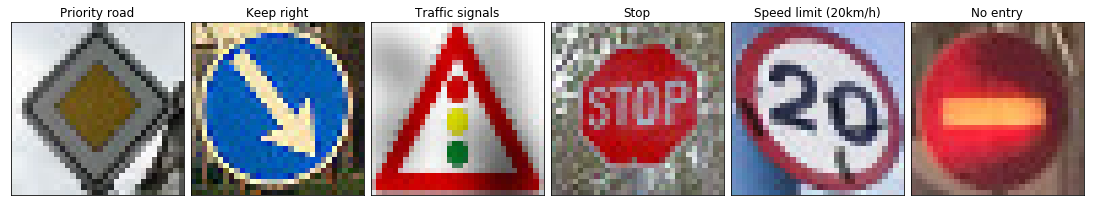
\includegraphics{./assets/chosen_images.png}
\caption{chosen\_images.png}
\end{figure}

\hypertarget{preprocessing-the-test-images}{%
\paragraph{Preprocessing the Test
Images}\label{preprocessing-the-test-images}}

We then proceeded to put the images into the \emph{preprocessing
pipeline}, were we got the enhanced, gray CALHE transformed, and
normalized representation of the images as shown below:

\begin{figure}
\centering
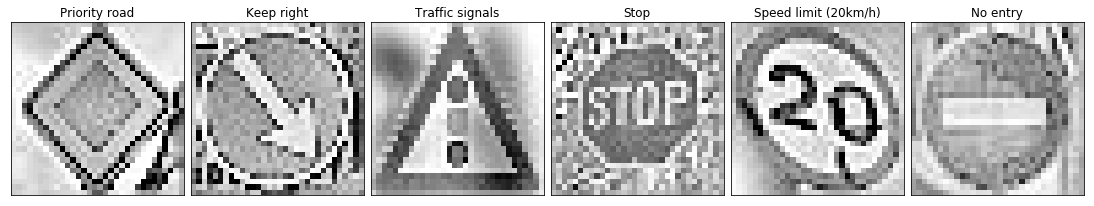
\includegraphics{./assets/preprocessed_test_images1.png}
\caption{preprocessed\_test\_images1.png}
\end{figure}

    \hypertarget{test-images-results}{%
\subsubsection{2. Test Images results}\label{test-images-results}}

\hypertarget{initial-results}{%
\paragraph{Initial Results}\label{initial-results}}

Here are the inference results on the \emph{6} test images:

\begin{longtable}[]{@{}ccc@{}}
\toprule
Prediction & True Class & Predicted Class\tabularnewline
\midrule
\endhead
{True} & Priority road & Priority road\tabularnewline
{True} & Keep right & Keep right\tabularnewline
{True} & Traffic signals & Traffic signals\tabularnewline
{True} & Stop & Stop\tabularnewline
{True} & Speed limit (20km/h) & Speed limit (20km/h)\tabularnewline
{True} & No entry & No entry\tabularnewline
\bottomrule
\end{longtable}

\begin{figure}
\centering
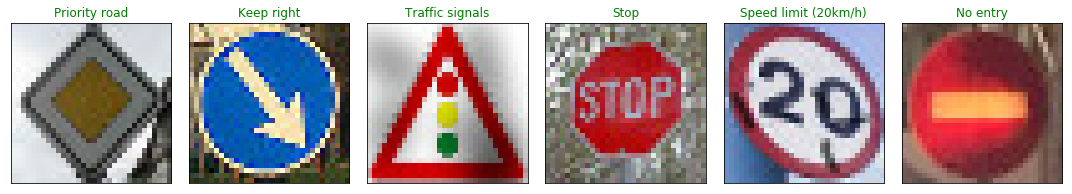
\includegraphics{./assets/test_images_redictions_1.png}
\caption{test\_images\_redictions\_1.png}
\end{figure}

So we got a \textbf{100\%} accuracy on these \emph{6} test images a
\textbf{2\%} increase over our dataset test accuracy of \textbf{98\%},
this might be because we're testing on a very small number of images
\textbf{6} images to be exact versus the \textbf{12,630} test set
images, so we're not encountering any of the \textbf{2\%} (252 images)
misclassified images we had for the test set.

This spurred my interest an we tested the model's prediction on more
test images either taken by my phone or from online images, we got
perfect results form most but we had some special cases that'll be shown
below.

    \hypertarget{especial-cases}{%
\paragraph{Especial cases}\label{especial-cases}}

\textbf{\texttt{MoNet0.1.4}}

We initially choose \texttt{0.1.4} as the best version for the model,
but after investigating on more test images model proved to produce poor
results for some signs like for the \textbf{End of no passing by
vehicles over 3.5 metric tons}.

\begin{figure}
\centering
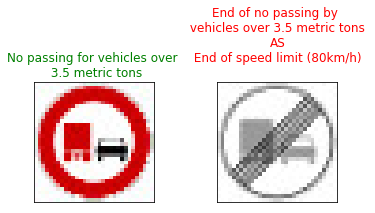
\includegraphics{./assets/esp1.png}
\caption{esp1.png}
\end{figure}

As we see here our \texttt{0.1.4} version misclassified \textbf{End of
passing by vehicles over 3.5 metric tons} as \textbf{End of speed limit
(80km/h)} which in all fairness bears a lot of similarity to, for both
of them are black and white and have lines going diagonally through
them.

\textbf{\texttt{MoNet0.1.5}}

Then we tried out the \texttt{0.1.5} to see effect of these two
mistrious signs: 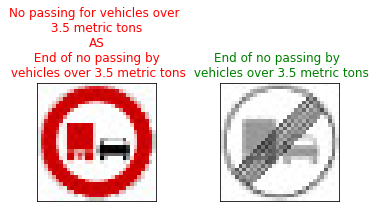
\includegraphics{./assets/esp2.png}

Version \texttt{0.1.5} does the opposite of \texttt{0.1.4} and it
falsely classifies \textbf{No passing by vehicles over 3.5 metric tons}
as \textbf{End of no passing by vehicles over 3.5 metric tons}, this
behaviour is rather peculiar because its virtually the same model with
the only difference being that \texttt{0.1.5} have been trained for a
couple of hundred epochs more. This suggests that each model overfit one
of the signs and ignored the other, its still a very strange case that
needs further investigation.

\textbf{\texttt{MoNet0.1.3}}

Finally we tried out the \texttt{0.1.3} version on the signs:

\begin{figure}
\centering
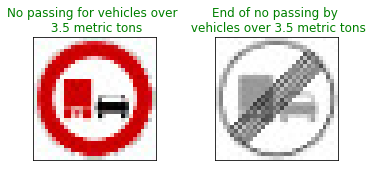
\includegraphics{./assets/esp3.png}
\caption{esp3.png}
\end{figure}

I ended up choosing the \texttt{MoNet0.1.3} due to its robust
classification of all test signs, in addition to its handling of this
especial case that baffled the other 2 variations. This variation also
gives better softmax predictions on the test images and on the
\textbf{UAE} test images that we'll see below.

    \hypertarget{softmax-probabilities} even, with others having less than an \texttt{0.1\%} for
other predictions. That might reflect that our model is too sure of its
results due the fact that it was trained on \texttt{70,879} over
\texttt{2000} epochs, I don't know if thats a good or a bad thing cause
for false classification as we'll see in the section below it gives a
very low value for the correct prediction too.

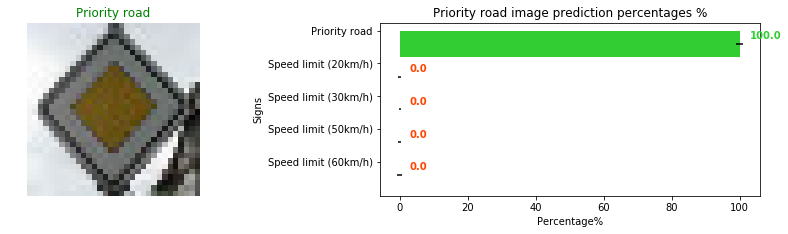
\includegraphics{./assets/sm1.png} 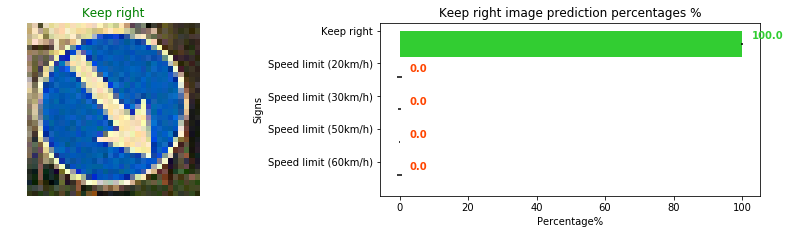
\includegraphics{./assets/sm2.png}
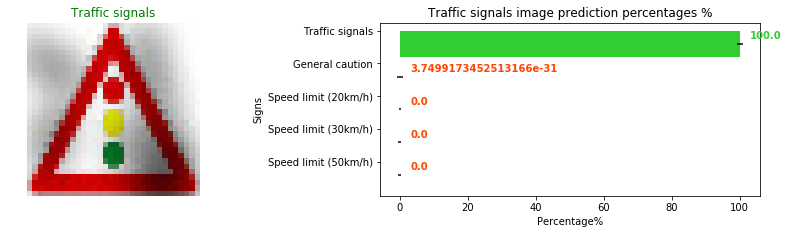
\includegraphics{./assets/sm3.png} 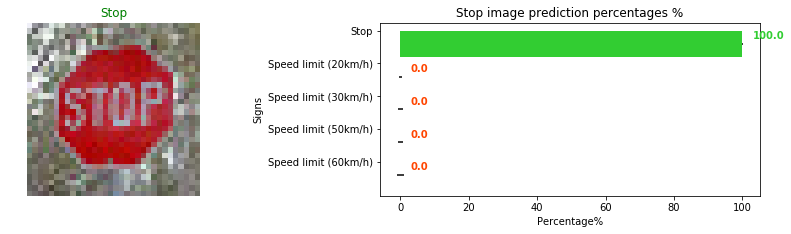
\includegraphics{./assets/sm4.png}
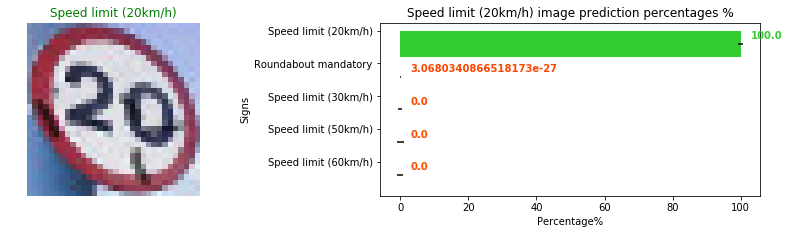
\includegraphics{./assets/sm5.png} 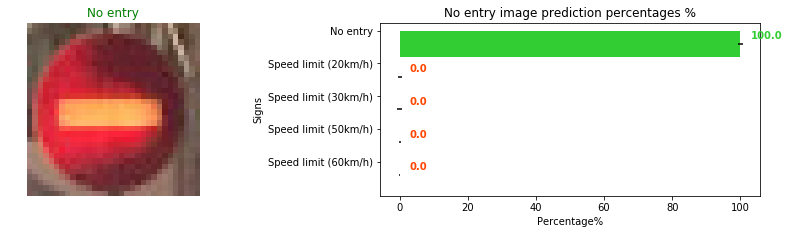
\includegraphics{./assets/sm6.png}

    \hypertarget{uae-traffic-signs-test}{%
\subsubsection{UAE Traffic Signs Test}\label{uae-traffic-signs-test}}

Here we needed to test what results our model will give on
\textbf{UAE(United Arab Emirates)} traffic signs that we took, some of
these signs have Arabic writing like the \textbf{Stop} sign, and others
are not in the original \textbf{German traffic signs} dataset like the
second image were we labeled it as \textbf{Right-of-way at the next
intersection} because its the closest counterpart in the dataset. We
also have the \textbf{Traffic signal} that looks close to the
\textbf{German sign} though the traffic lights are bordered by a black
rectangular shape rather than white.

\begin{figure}
\centering
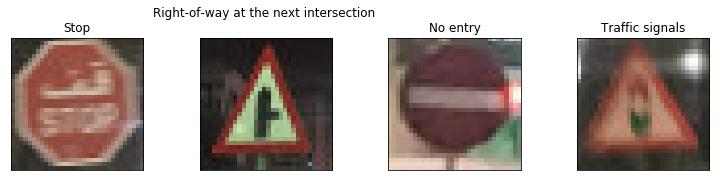
\includegraphics{./assets/uae_test_iamges.png}
\caption{uae\_test\_iamges.png}
\end{figure}

\begin{figure}
\centering
\includegraphics{attachment:uae_test_images_calhe.png}
\caption{uae\_test\_images\_calhe.png}
\end{figure}

\begin{longtable}[]{@{}ccc@{}}
\toprule
\begin{minipage}[b]{0.14\columnwidth}\centering
Prediction\strut
\end{minipage} & \begin{minipage}[b]{0.37\columnwidth}\centering
True Class\strut
\end{minipage} & \begin{minipage}[b]{0.40\columnwidth}\centering
Predicted Class\strut
\end{minipage}\tabularnewline
\midrule
\endhead
\begin{minipage}[t]{0.14\columnwidth}\centering
{False}\strut
\end{minipage} & \begin{minipage}[t]{0.37\columnwidth}\centering
Stop\strut
\end{minipage} & \begin{minipage}[t]{0.40\columnwidth}\centering
No entry\strut
\end{minipage}\tabularnewline
\begin{minipage}[t]{0.14\columnwidth}\centering
{True}\strut
\end{minipage} & \begin{minipage}[t]{0.37\columnwidth}\centering
Right-of-way at the next intersection\strut
\end{minipage} & \begin{minipage}[t]{0.40\columnwidth}\centering
Right-of-way at the next intersection\strut
\end{minipage}\tabularnewline
\begin{minipage}[t]{0.14\columnwidth}\centering
{True}\strut
\end{minipage} & \begin{minipage}[t]{0.37\columnwidth}\centering
No entry\strut
\end{minipage} & \begin{minipage}[t]{0.40\columnwidth}\centering
No entry\strut
\end{minipage}\tabularnewline
\begin{minipage}[t]{0.14\columnwidth}\centering
{False}\strut
\end{minipage} & \begin{minipage}[t]{0.37\columnwidth}\centering
Traffic signals\strut
\end{minipage} & \begin{minipage}[t]{0.40\columnwidth}\centering
Beware of ice/snow\strut
\end{minipage}\tabularnewline
\bottomrule
\end{longtable}

\begin{figure}
\centering
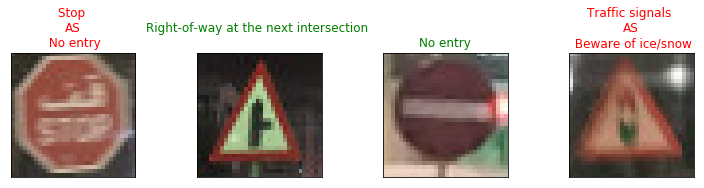
\includegraphics{./assets/uae_test_images_predictions.png}
\caption{uae\_test\_images\_predictions.png}
\end{figure}

As we can see we go a \textbf{50\%} accuracy on these \textbf{4} images,
the images that closely resembled the \textbf{German} signs were
correctly classified; however, the \textbf{Stop} sign which has the same
edges as the original dataset was misclassified, maybe thats because the
classifier pays more consideration to the content inside the sign edges.

Here are the top \texttt{5} Softmax predictions for each of the
\textbf{UAE} signs:

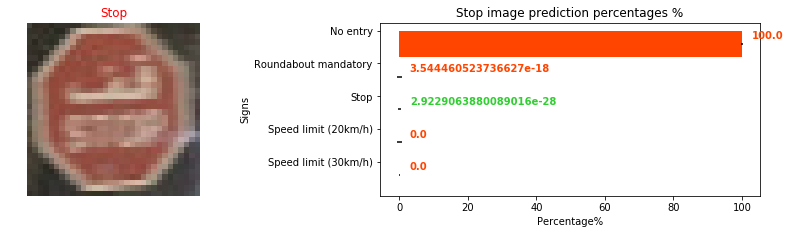
\includegraphics{./assets/uae_sm1.png}
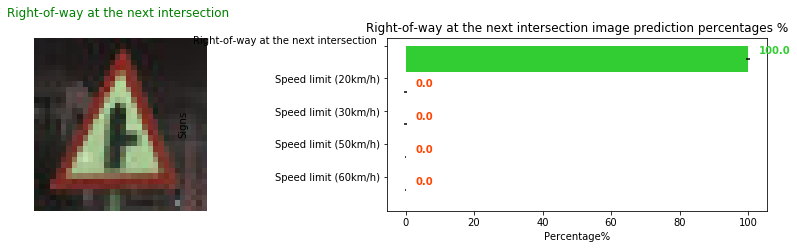
\includegraphics{./assets/uae_sm2.png}
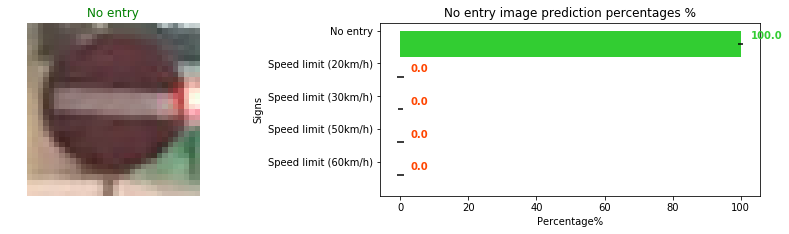
\includegraphics{./assets/uae_sm3.png}
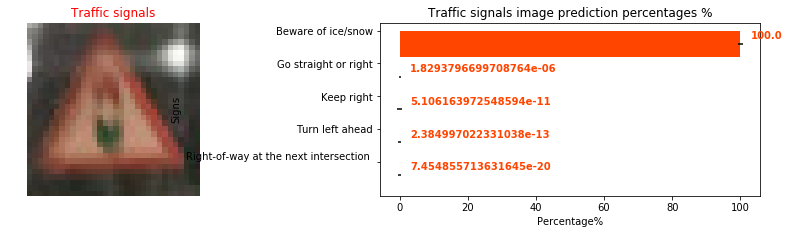
\includegraphics{./assets/uae_sm4.png}

    As we can see trend of getting near \texttt{100\%} prediction is
continuing here even for the misclassified signs; we got the right
prediction for the \textbf{Stop} sign as the third Softmax minuscule
prediction of \texttt{2.9229063880089016e-28\%}. In the case of the
\textbf{Traffic signals} we didn't get the correct label in any of the
Softmax predictions, but we got all of the triangular signs in the top
\texttt{5} predictions except for the \textbf{Traffic signals} which
means that the network could identify the sign's shape but failed to
classify the figure inside.

    \hypertarget{visualizing-the-neural-network}{%
\subsection{Visualizing the Neural
Network}\label{visualizing-the-neural-network}}

Here we'll visualize the neural network's 3 \texttt{convolutional}
layers' activations and discuss how the network captures information
from a stimuli image. All these activations were taken before the
trailing \texttt{maxpooling} layer.

\hypertarget{first-convolutional-layer}{%
\subsubsection{First Convolutional
Layer}\label{first-convolutional-layer}}

\begin{figure}
\centering
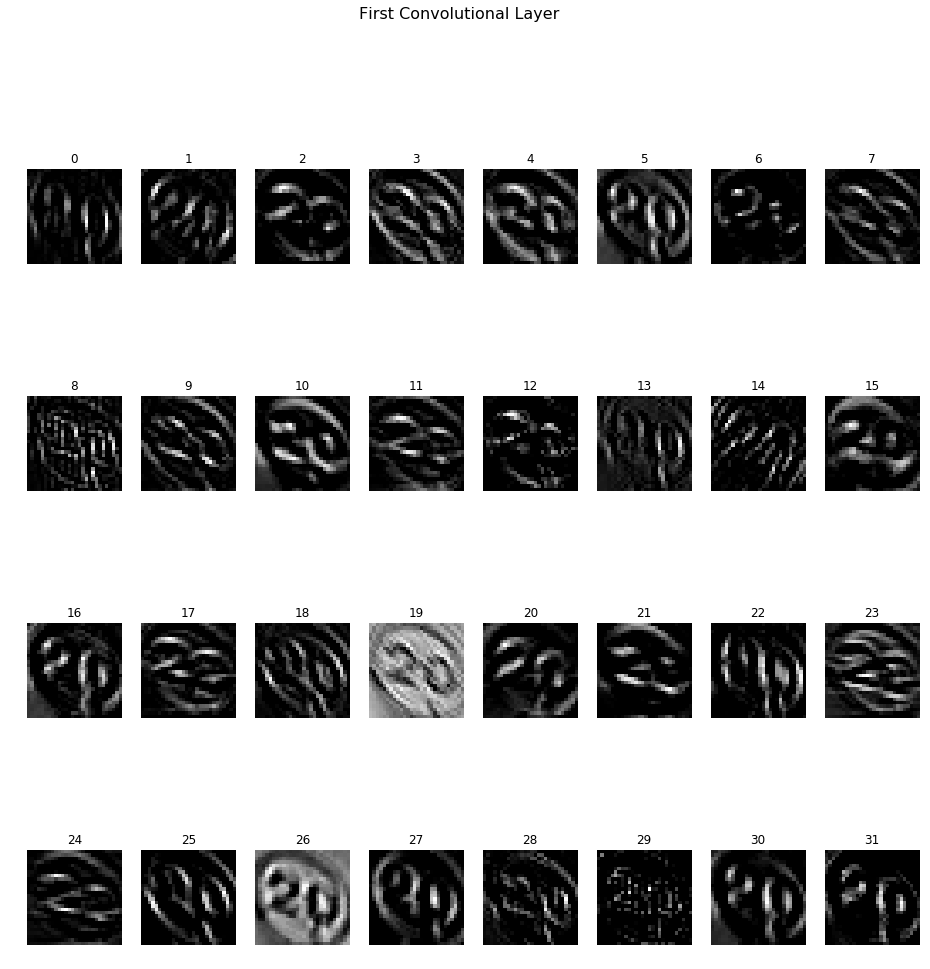
\includegraphics{./assets/conv1.png}
\caption{conv1\_activation.png}
\end{figure}

So here we have the \texttt{MoNet0.1.3} First Convolutional Layer
resulting filters, we can see that the each of the 32 filters captures
the curves and edges of the \textbf{Speed limit (20 km/h)}. Mainly the
filters focus on the edges of the sign and the edges of the digits
inside while ignoring whats outside all together. Some of the filters
even capture the \emph{graffiti} but not to a high degree, other filters
like filter \emph{17} is capturing some noisy representation of the
sign.

\hypertarget{second-convolutional-layer}{%
\subsubsection{Second Convolutional
Layer}\label{second-convolutional-layer}}

\begin{figure}
\centering
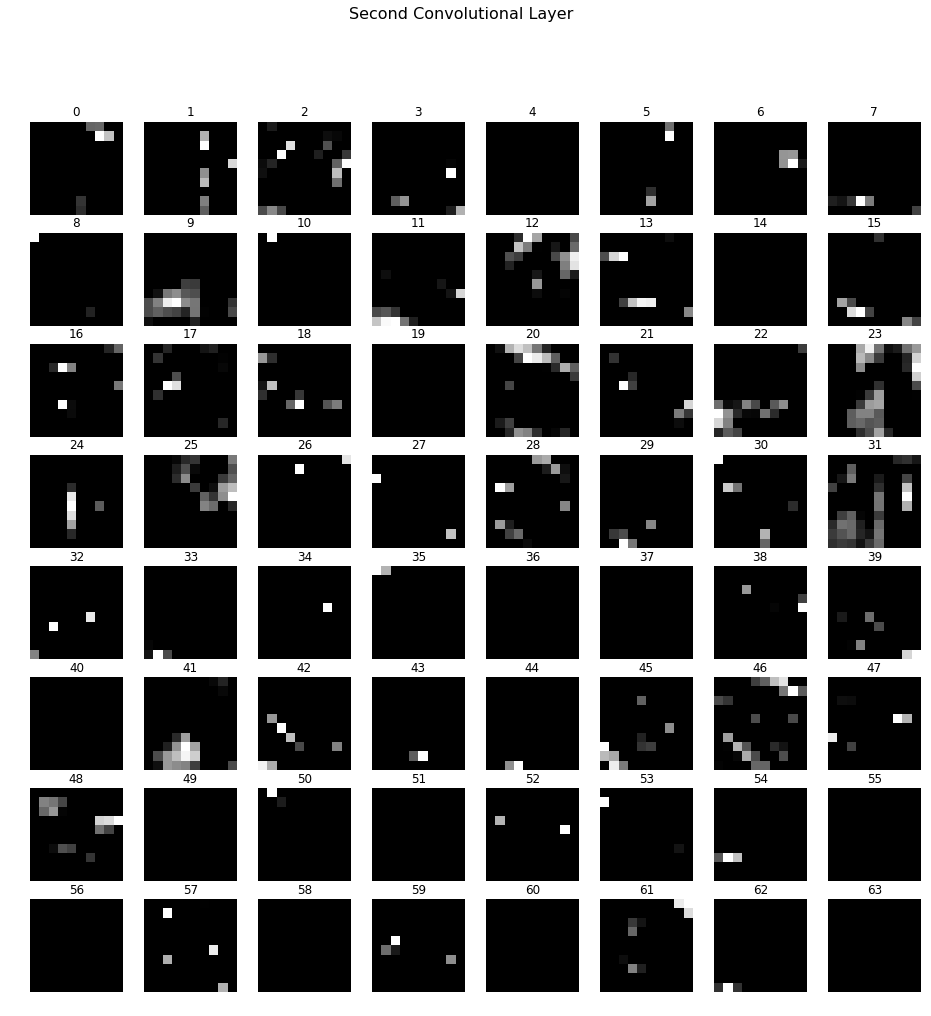
\includegraphics{./assets/conv2.png}
\caption{conv2\_activation.png}
\end{figure}

Here in the \texttt{second\ layer} we have \texttt{64} filters and a
\texttt{10x10} image, as we can see its really hard to clearly identify
the features captured, but we can make out some features like the sign
edges like in \emph{41} which shows the lower edges and some filters
contain the digit edges as in the case of \emph{23}.

\hypertarget{last-convolutional-layer}{%
\subsubsection{Last Convolutional
Layer}\label{last-convolutional-layer}}

\begin{figure}
\centering
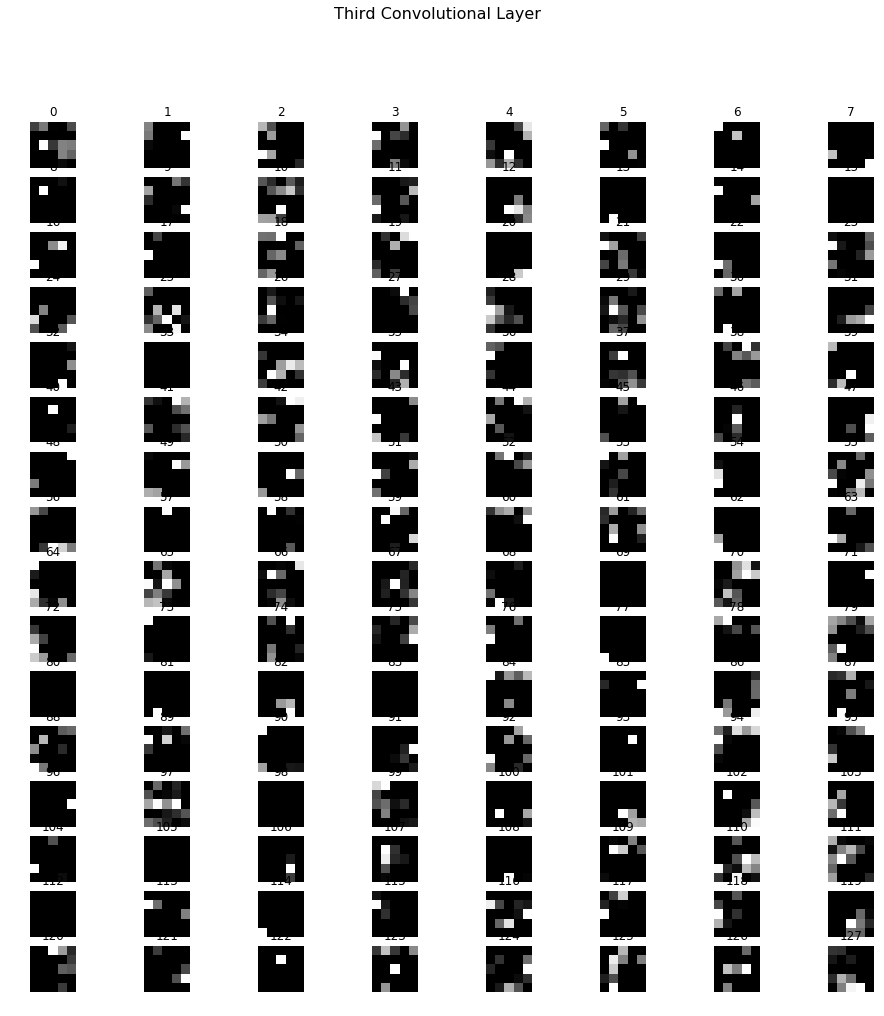
\includegraphics{./assets/conv3.png}
\caption{conv3\_activation.png}
\end{figure}

As we dive deeper the features become human unreadable cause our image
size decreases and our feature size increases; however, its obvious that
our network is still capturing plenty of information in its \texttt{128}
features. We might event still see some small resemblance to the sign's
curved edges.

    \hypertarget{conclusion}{%
\subsection{\#\# Conclusion}\label{conclusion}}

First I'd like to thank you for reading and hope you learned something
from this project cause I sure did. In the course of this project I've
learned a lot about constructing a robust classifier and preparing its
training data. I've executed many tests and looked at many graphs which
gave me an understanding of how certain techniques alone or in
combination with others affect the model; for example applying
\textbf{normalization} helps the network learn faster, \textbf{dropout}
combined with a higher number of epochs gives better results and
prevents overfitting to a degree, and \textbf{data augmentation} and the
relative approach used in the project helps the network learn better and
it rockets the accuracy up (well just \texttt{2-3\%} but its good
enough). This was a really fun project and I enjoyed working on it way
much than I should cause it took me a lot of time to finish, but it was
a great experience and hopefully I'll come back to it and improve a lot
more upon it and get the accuracy a bit higher.

    \hypertarget{potential-shortcomings} 2. \textbf{RGBG} gives bad results, but it should give
more information. 3. Model \texttt{0.1.4} and \texttt{0.1.5} especial
case weird behaviour need further investigation.

    \hypertarget{suggested-solutions}{%
\subsection{Suggested Solutions}\label{suggested-solutions}}

\begin{enumerate}
\def\labelenumi{\arabic{enumi}.}
\tightlist
\item
  Better augmentation algorithm to increase the dataset size and still
  gives us a uniform dataset.
\item
  Maybe in order for the \textbf{RGBG} combo to work I need to have a
  deeper network.
\item
  Further investigation in some of the model variations
\end{enumerate}

    \hypertarget{future-improvements-and-projects}{%
\subsection{Future Improvements and
Projects}\label{future-improvements-and-projects}}

\begin{itemize}
\tightlist
\item
  I'm planning to build a traffic signs recognizer and combine it with
  the classifier to have a fully fledged traffic signs classifier, I'm
  planning on doing this in a mobile app so it can be easily used for
  testing.
\item
  I'm also planning to further explore the idea and use the model on the
  \textbf{UAE} traffic signs and see if I can achieve closer result to
  the \textbf{German} traffic signs dataset.
\item
  I also want to try batch normalization, I already tried it many times
  in the project but I got very bad result, so I'll try it out again
  sometime in the future.
\end{itemize}

Please share with me any shortcomings you've notices or improvements
that I can apply or may help in future projects, your advice is deeply
appreciated. :)


    % Add a bibliography block to the postdoc
    
    
    
    \end{document}
